\documentclass[
  aspectratio=169,
]{beamer}
\usepackage{algorithm}
\usepackage{algorithmic}
\usepackage[spanish]{babel}
\usepackage[utf8]{inputenc}
\usepackage[T1]{fontenc}
\usepackage{booktabs}
\usepackage{amsmath}
\usepackage{mathtools}
\usepackage{subfigure}
\usepackage{hyperref}
\usepackage{xcolor}
\usetheme[
  workplace=teiresias,
]{MU}

\graphicspath{{./imagenes/ResultadosNumericos/RightAngeCantilever/},{./imagenes/ResultadosNumericos/CantieleverPendulum/},{./imagenes/ResultadosNumericos/SimpleCable/},{./imagenes/ResultadosNumericos/TransmissionTormenta/}, {./imagenes/Preliminares/Corrotacional/},{./imagenes/Preliminares/deslizamientoRelativo/},{./imagenes/ResultadosNumericos/uniformCantilever/},{./imagenes/Metodologia/},{/imagenes/Anexo/}{./imagenes/Introduccion/}}


%%%%%%%%%%%%%%%%%%%%%%%%%%%%%%%%%%%%%%%%%%% BEGIN DOCUMENT %%%%%%%%%%%%%%%%%%%%%%%%%%%%%%%%%%%%%
 \begin{document}
	\begin{small}

\title[Maestría en Ingeniería Estructural]{Implementación de una formulación corrotacional en dinámica no lineal y aplicación al modelado de líneas de transmisión eléctrica }
%\subtitle[Short Presentation Subtitle]{Full Presentation Subtitle}
\author[M.C. Vanzulli]{Autor: M.C. Vanzulli$^\text{IIMPI}$  \\Director de tesis: J.M. Pérez Zerpa$^\text{IET}$ \\ Director académico: G Usera$^\text{IIMPI}$ }
\institute [IIMPI-IET]{1-Instituto de Ingeniería Mecánica y Producción Industrial, Facultad de Ingeniería, UdelaR \\ 2-Instituto de Estructuras y Transporte, Facultad de Ingeniería UdelaR  }
\date{\today}
\keywords{Formulación corrotacional; Método de los Elementos Finitos; Dinámica estructural; Transmisión eléctrica}

%%%%%%%%%%%%%%%%%%%%%%%%%%%%%%%%%%    FRAME   %%%%%%%%%%%%%%%%%%%%%%%%%%%%%%%%%%%
\begin{frame}[plain]
\maketitle
\end{frame}
%%%%%%%%%%%%%%%%%%%%%%%%%%%%%%%%%%    FRAME   %%%%%%%%%%%%%%%%%%%%%%%%%%%%%%%%%%%
\begin{frame}{Tabla de contenidos:}
	\tableofcontents
\end{frame}
%%%%%%%%%%%%%%%%%%%%%%%%%%%%%%%%%%%%%%%%     SECTION  %%%%%%%%%%%%%%%%%%%%%%%%%%%%%%%%%%%%%%%%%
\section[Introducción y preliminares]{Introducción y preliminares}
\AtBeginSection[]
{
	\begin{frame}
		\frametitle{Metodología}
		\tableofcontents[currentsection]
	\end{frame}
}
%%%%%%%%%%%%%%%%%%%%%%%%%%%%%%%%%%    SUBSECTION   %%%%%%%%%%%%%%%%%%%%%%%%%%%%%%%%%%%
\subsection[Agradecimientos]{Agradecimientos}
\begin{frame}{Agradecimientos:}{}
	\begin{block}{Gracias a:}
	\begin{itemize}
%		\item Mis amigos y familia por su apoyo.
%		\pause 
%		\item A mi novia Flor por ser un alero cuando llueve y dos alas cuando hay sol. 
%		\pause
		\item Mis tutores de la Facutlad de Ingeniería UdelaR por guiarme en este proceso de aprendizaje.
		\pause
		\item La \emph{Comisión Académica de Posgrado} por financiar este proyecto y permitirme dedicarme a la investigación.
		\pause
		\item Mis compañeros de trabajo por cuestionarme, impulsarme y hacer reír al malhumor.  
	\end{itemize}
	\end{block}
\end{frame}
%%%%%%%%%%%%%%%%%%%%%%%%%%%%%%%%%%    SUBSECTION   %%%%%%%%%%%%%%%%%%%%%%%%%%%%%%%%%%%
\subsection[Introducción]{Introducción}
%%%%%%%%%%%%%%%%%%%%%%%%%%%%%%%%%%    FRAME   %%%%%%%%%%%%%%%%%%%%%%%%%%%%%%%%%%%
\begin{frame}
	\begin{block}{Motivación internaciónal:}
		\begin{itemize}
			\item En Australia el 90\% de las torres de alta tensión dañadas fallaron debido a fenómenos de tormentas severas.  {\color{blue}(Li,2000)}
			\pause
			\item 55 torres de alta tensión fueron \alert{destruidas} en Chubut en el año 2020.
			\pause
		\end{itemize}
	\end{block}
	\vfill
	\begin{block}{Motivación local:}
		\begin{itemize}
			\item El 10 de marzo de 2002 azotó una tormenta devastadora, con velocidades de ráfaga desmesuradas provocando el \alert{colapso} de 67 torres eléctricas.
			\pause
			\item Se destinaron \alert{12 millones de USD} a cubrir las perdidas y daños al servicio de distribución eléctrica. {\color{blue}(Durañona,2019)}
			\pause
			\item Se registraron más de veinte eventos de desconexión en el periodo de 2000-2007 en la línea de alta tensión Palmar-Montevideo.
		\end{itemize}
	\end{block}
\end{frame}

%%%%%%%%%%%%%%%%%%%%%%%%%%%%%%%%%%    FRAME   %%%%%%%%%%%%%%%%%%%%%%%%%%%%%%%%%%%
\begin{frame}{Problema:}{}
	\begin{figure}[htbp]
		\centering
		\subfigure[Ilustración de balanceos excesivos torre Ruta 5. ]{	\def\svgwidth{35mm}
			\input{./imagenes/Introduccion/Torre.pdf_tex}}
		\subfigure[Colapso de torre en Chubut-Argentina, 2020 \href{https://www.clarin.com/sociedad/fenomeno-galloping-cayeron-torres-alta-tension-patagonia_0_fc3FYz1O-.html}{\structure{Noticia Clarín}}]{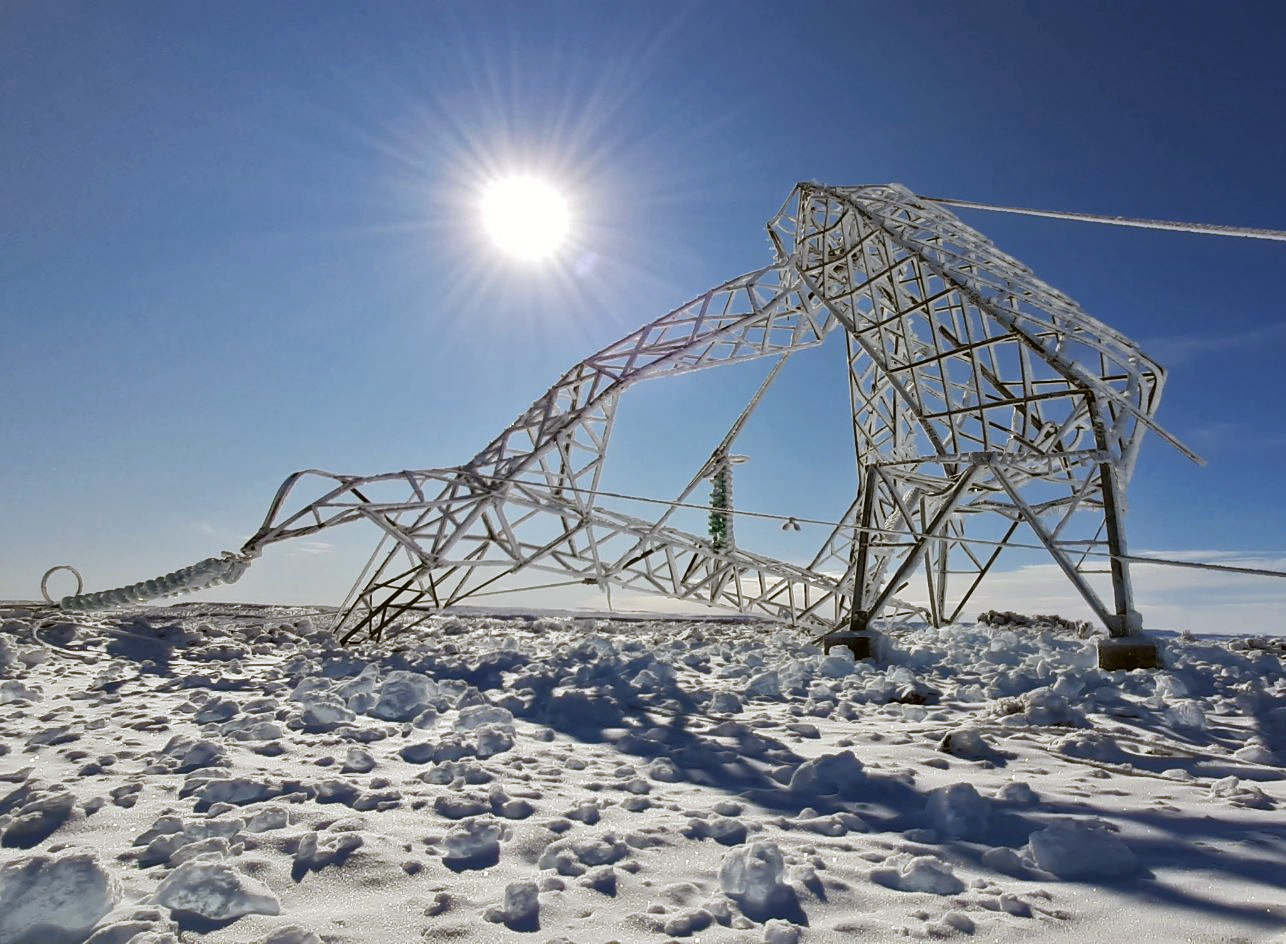
\includegraphics[width=0.45\textwidth]{./imagenes/Introduccion/TorreColapsada.jpg}}
	\end{figure}
\end{frame}

%%%%%%%%%%%%%%%%%%%%%%%%%%%%%%%%%%    FRAME   %%%%%%%%%%%%%%%%%%%%%%%%%%%%%%%%%%%
\begin{frame}{Tormentas convectivas:}{}
	
	\begin{figure}[htbp]
		\centering
		\includegraphics[width=1\textwidth]{./imagenes/Introduccion/ilusTormentasConvectivas.png}
		\caption{Esquema de tormentas convectivas extraído de \href{https://www.britannica.com/science/thunderstorm}{\structure{Encyclopedia britannica}}}
	\end{figure}
\end{frame}
% Agregar las causas


%%%%%%%%%%%%%%%%%%%%%%%%%%%%%%%%%%    FRAME   %%%%%%%%%%%%%%%%%%%%%%%%%%%%%%%%%%%
\begin{frame}{Tormentas en Uruguay:}{}
\vspace{-.5cm}	
	\begin{figure}[htbp]
	\centering
	\subfigure[Foto de tormenta convectiva en Cabo Polonio \href{https://www.inumet.gub.uy/mapa-interactivo}{\structure{INUMET}}]
	{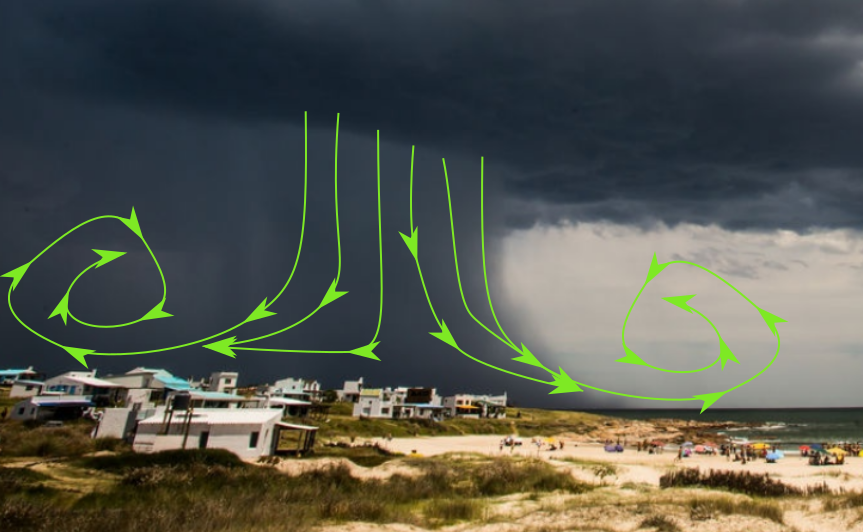
\includegraphics[width=0.5\textwidth]{./imagenes/Introduccion/TormentaPolonio.png}}
	\subfigure[Tormenta convectiva publicada en \color{blue}(Viera,1969)]
	{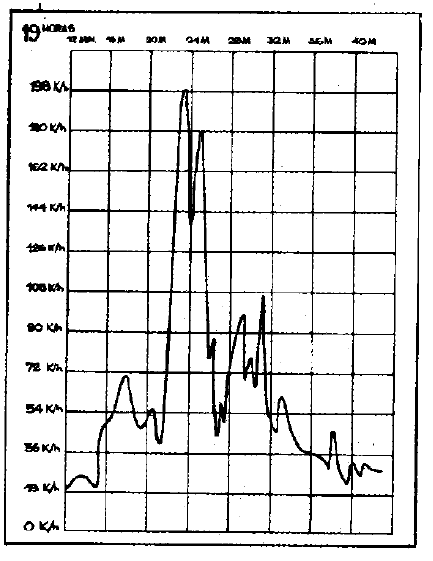
\includegraphics[width=0.25\textwidth]{./imagenes/Introduccion/tormentaMontevideo.png}}
	\end{figure}
\vspace{-.25cm}
%\pause
\begin{alertblock}{¡Cambio climático!}
	Según {\color{blue}(Brook,2013)} este agudiza la intensidad y frecuencia de tormentas convectivas.
\end{alertblock}
\end{frame}


%%%%%%%%%%%%%%%%%%%%%%%%%%%%%%%%%%    FRAME   %%%%%%%%%%%%%%%%%%%%%%%%%%%%%%%%%%%
\begin{frame}{Enfoque:}{}
	\begin{block}{¿Cómo?}
		\begin{itemize}
			\item Se estudiaron diferentes ejes temáticos que involucra el fenómeno. Se exploraron distintas formulaciones para el modelado de líneas eléctricas. 
			\item Se eligió la metodología corrotacional de vigas 3D presentada en {\color{blue}(Le,2014)}, debido a sus atractivos para el modelado de estructuras con movimientos de gran amplitud.
			%Los autores de la literatura han acuñado sus investigaciones en diversios tipos de elementos. Utilizando elementos de barras se destacan los autores: \cite{desai1995finite}, \cite{yan2009numerical}, \cite{gani2010dynamic} y \cite{yang2016nonlinear}. A pesar de la gran esbeltez de las líneas de transmisión eléctrica, las mismas cuentan con rigidez a flexión. Los elementos de barra no son capaces de representarla, por ende, es necesario incorporar elementos de vigas tridimensionales. Debido a los grandes desplazamientos y rotaciones que se presentan durante las trayectorias en tormentas, se implementó una formulación corrotacional considerando la dinámica del problema.

			\item Se agregaron componentes aerodinámicos lineales debido a la interacción sólido-fluido.
			%El campo de la metodología corrotacional es muy amplio, pero debido a la claridad y contemporaneidad en el desarrollo de sus publicaciones, se tomo como principal referencia de la formulación \citep{Le2014}. A esta se le agregaron componentes no lineales debido a la interacción del sólido en un fluido que ejerce determinadas fuerzas. 
			\item Se implementó esta formulación en la herramienta de código abierto \href{https://github.com/ONSAS/ONSAS.m}{\emph{Open Nonlinear Structural Analysis Solver}}.
			\item Se desarrollaron tres modelos computacionales validando la formulación y aplicando la implementación a sistemas de transmisión eléctrica.  
		\end{itemize}
	\end{block}	
\end{frame}
%%%%%%%%%%%%%%%%%%%%%%%%%%%%%%%%%%    SUBSECTION   %%%%%%%%%%%%%%%%%%%%%%%%%%%%%%%%%%%
\subsection[Preliminares]{Preliminares}
%%%%%%%%%%%%%%%%%%%%%%%%%%%%%%%%%%%%%%%%FRAME%%%%%%%%%%%%%%%%%%%%%%%%%%%%%%%%%%%%%%%%%
\begin{frame}{Componentes del sistema:}{}
	\vspace{-.5cm}	
	\setcounter{figure}{0}
	\begin{figure}[htbp]
		\centering
		\subfigure[Ilustración conductores norma IEC 60183 y ensayo MT UTE.]
		{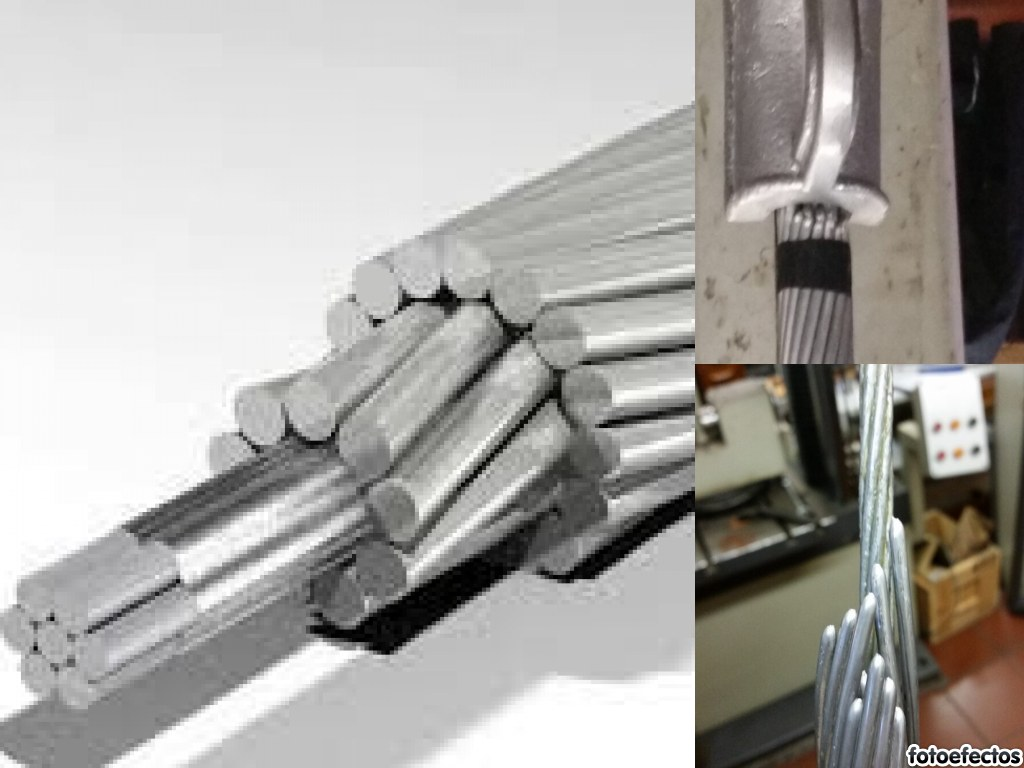
\includegraphics[width=0.42\textwidth]{./imagenes/Metodologia/Conductores.jpg}}
		\subfigure[Aisladores de alta tnesión. ]
		{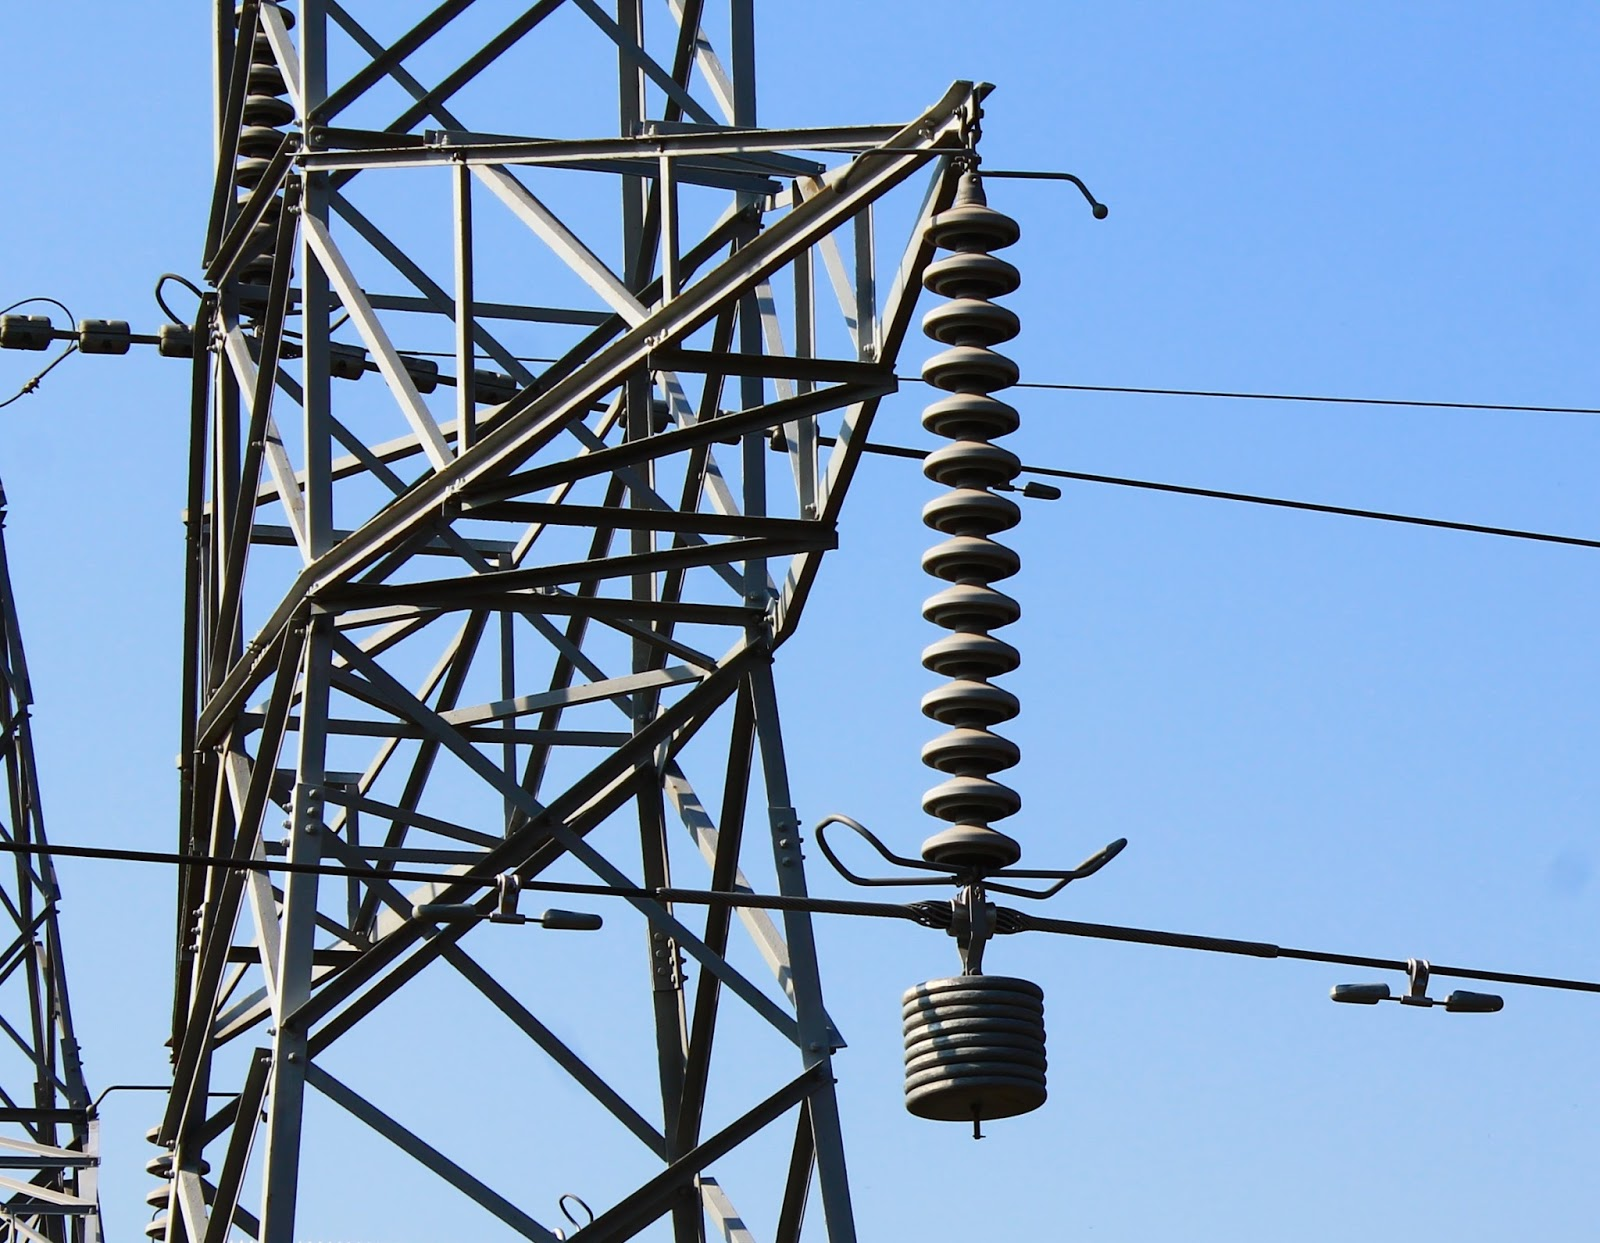
\includegraphics[width=0.42\textwidth]{./imagenes/Metodologia/CadenasAisladoras.jpg}}
	\end{figure}
\end{frame}
%%%%%%%%%%%%%%%%%%%%%%%%%%%%%%%%%%%%%%%%FRAME%%%%%%%%%%%%%%%%%%%%%%%%%%%%%%%%%%%%%%%%%
\begin{frame}{Deslizamiento en conductores:}{}
	\setcounter{figure}{0}
  	Según {\color{blue}(Foti,2016)} existe un comportamiento de \alert{hysterisis no lineal} al interior del conductor...

	\begin{figure}[htbp]
		\centering
		\subfigure[Modelo de contacto diferenicial]
		{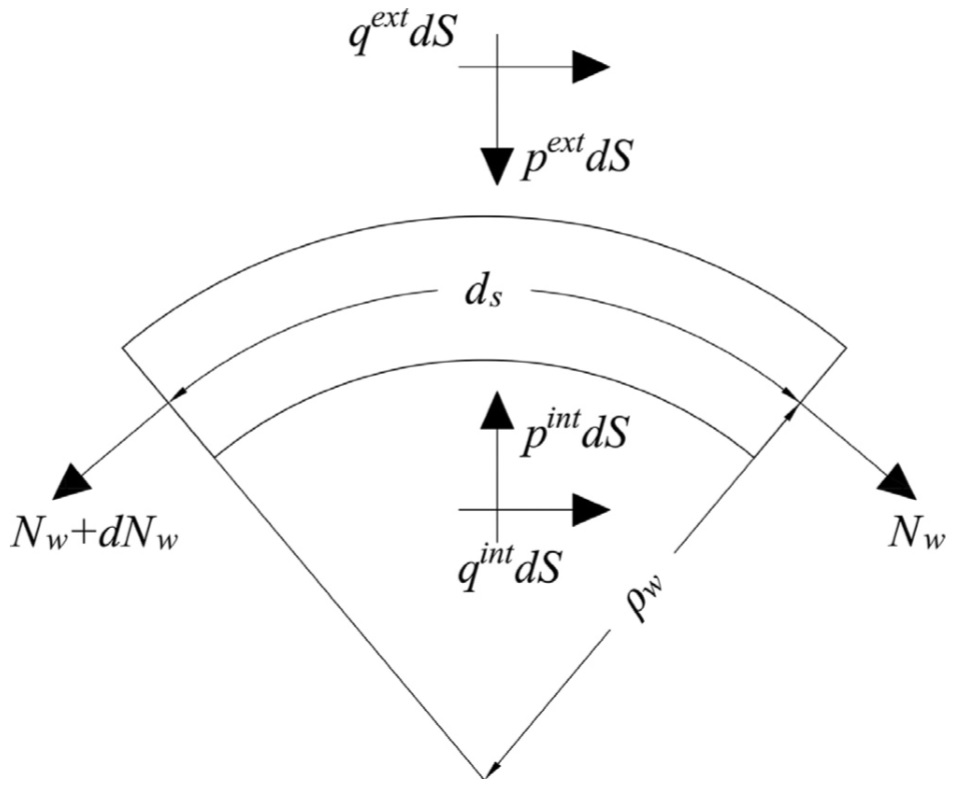
\includegraphics[width=0.45\textwidth]{./imagenes/Preliminares/deslizamientoRelativo/Contacto.jpg}}
		\subfigure[Límite de tensión no lineal para diferntes curvaturas.]
		{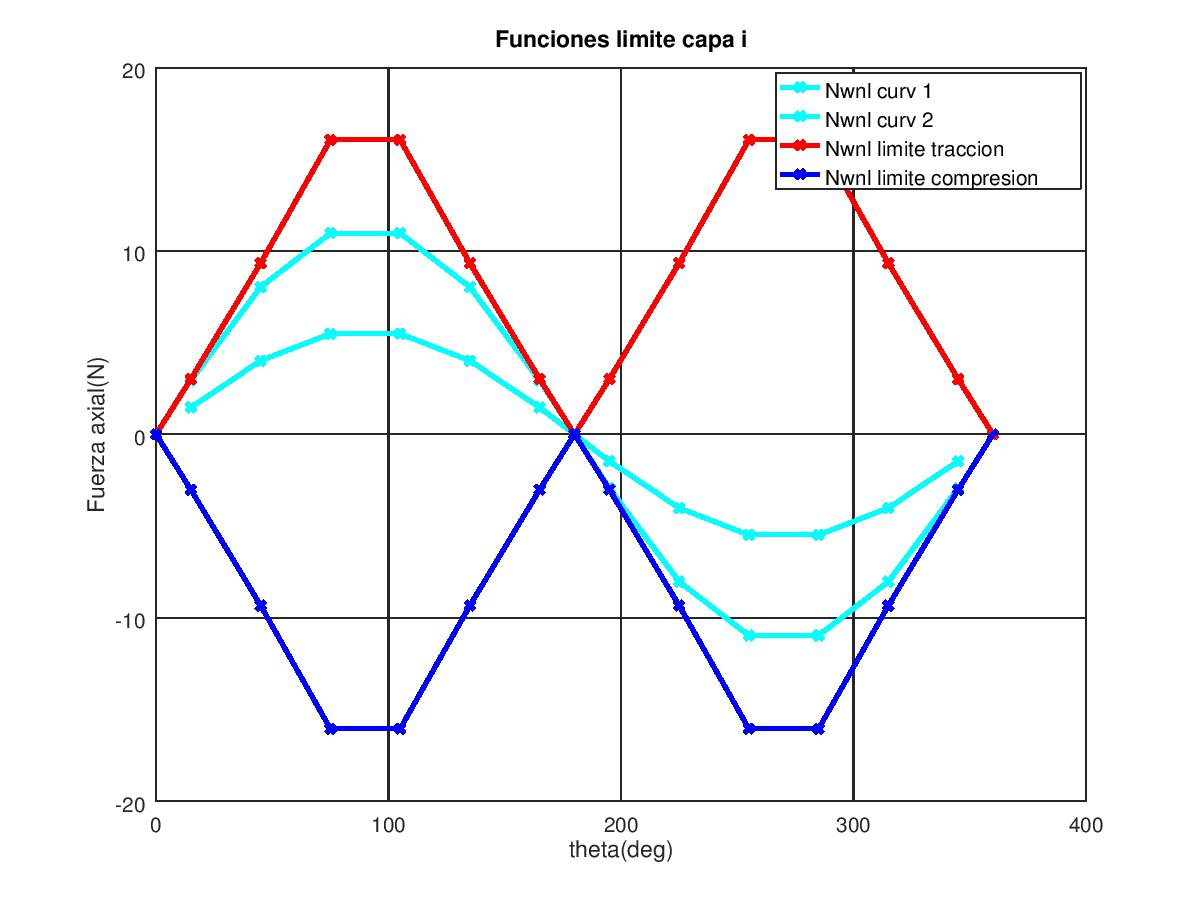
\includegraphics[width=0.5\textwidth]{./imagenes/Preliminares/deslizamientoRelativo/Superpuesto.jpg}}
	\end{figure}
\end{frame}

\begin{frame}{Elementos de barra reticulados:}{}
%Los autores de la literatura han acuñado sus investigaciones en diversios tipos de elementos. Utilizando elementos de barras se destacan los autores: \cite{desai1995finite}, \cite{yan2009numerical}, \cite{gani2010dynamic} y \cite{yang2016nonlinear}. A pesar de la gran esbeltez de las líneas de transmisión eléctrica, las mismas cuentan con rigidez a flexión. Los elementos de barra no son capaces de representarla, por ende, es necesario incorporar elementos de vigas tridimensionales. Debido a los grandes desplazamientos y rotaciones que se presentan durante las trayectorias en tormentas, se implementó una formulación corrotacional considerando la dinámica del problema.

	\begin{figure}[htbp]
		\centering
		\subfigure[Modelo de un conductor conisderando elementos de barra.]
		{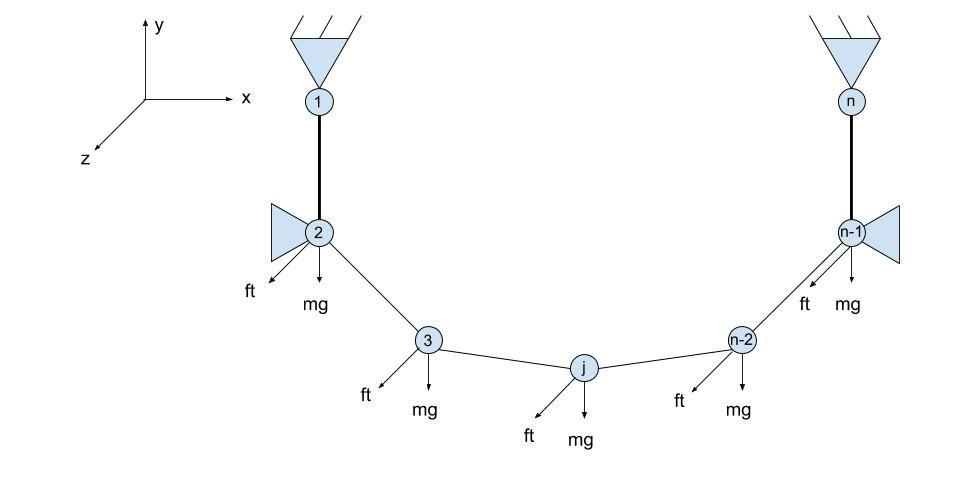
\includegraphics[width=0.4\textwidth]{./imagenes/Introduccion/trussModel/Model.jpg}}
		\subfigure[Resultados del ángulo de balanceo.]
		{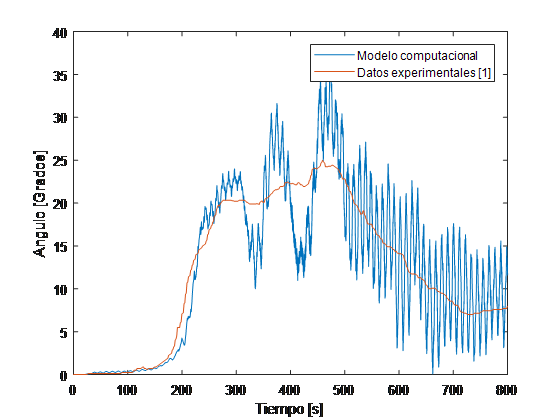
\includegraphics[width=0.4\textwidth]{./imagenes/Introduccion/trussModel/Angle.png}}
	\end{figure}
%Conclusiones del trabajo:
% Para cargas uniformes en el eje axial el modelo 2D del pendulo dinámico es válido e igual al 3D.
% se analizó uana solucipon de masas concentradas de 10Kg a 1/6 de distancia no presentandose significativas diferencias de las frecuencias.
% Estas rondan 0.09Hz
% Existe una inestabilidad numñerica del modelo con la felxión relativa entre los elementos asociada a la falta de rigidez en la formulación, entonces...

	
\end{frame}
%%%%%%%%%%%%%%%%%%%%%%%%%%%%%%%%%%%%%%%%FRAME%%%%%%%%%%%%%%%%%%%%%%%%%%%%%%%%%%%%%%%%%
\begin{frame}{Equilibrio de fuerzas:}{}
	%Aplicando d' almebertDiscretizando el cuerpo mediante el MEF, para cada nodo y en cada instante, debe cumplirse el balance vectorial entre fuerzas internas $\bf{f}_{int}$, inerciales $\bf{f}_{ine}$ y externas $\bf{f}_{ext}$. 
	%Aparece un término aerodinámico \gls{FuerzaViscosa} que depende de la velocidad lineal del rígido. Este término debe tratarse aparte ya que su naturaleza, a pesar de ser externa, es una función de el estado cinemático del sólido. La ecuación de equilibrio de fuerzas en el instante $t+\delta_t$ resulta:
	\begin{block}{Ecuación de equilibrio no lineal:}
		\begin{equation}\label{Eq:MET:EquilibrioExacto}
				\bf{f}_{ext,t+\delta_t}-\bf{f}_{int,t+\delta_t}-\bf{f}_{ine,t+\delta_t}=0
		\end{equation}
	\end{block}
%	\begin{block}{Métodos iterativos:}
%	\begin{equation}\label{Eq:MET:Resto}
%		\begin{split}
%			\bf{r}(\bf{d}_{t+\\delta_t})&=(-\bf{f}_{ext,t+\delta_t}+\bf{f}_{int}(\bf{d}_{t+\delta_t})+\bf{f}_{vis}(\dot{\bf{d}}_{t+\delta_t})...\\	
%			&...+\bf{f}_{ine}(\bf{d_{t+\delta_t}},\dot{\bf{d}}_{t+\delta_t}(d_{t+\delta_t},\bf{d_t},\bf{\dot{d}_t},\bf{\ddot{d}_t}),
%			\ddot{\bf{d}}_{t+\delta_t}(d_{t+\delta_t},\bf{d_t},\bf{\dot{d}_t},\bf{\ddot{d}_t}))
%			\approx 0
%		\end{split}
%	\end{equation}
%	\end{block}
%Los metodos iterativos para funciones vectoriales no lineales como ser el de Newton porponen una iteración en k se aproxima a la solución y el vector de fuerzas no será nula sino igual a un residuo:
%\pause
\vfill
\begin{block}{Métodos iterativos:}
	\begin{equation}\label{Eq:MET:Resto}
		\begin{split}
			\bf{r}(\bf{d}_{t+\delta_t})&=(-\bf{f}_{ext,t+\delta_t}+\bf{f}_{int}(\bf{d}_{t+\delta_t})+...\\	
			&...+\bf{f}_{ine}(\bf{d_{t+\delta_t}},\bf{v}_{t+\delta_t}(d_{t+\delta_t},\bf{d_t},\bf{v_t},\bf{a_t}),
			\bf{a}_{t+\delta_t}(d_{t+\delta_t},\bf{d_t},\bf{v_t},\bf{a_t}))
			\approx 0
		\end{split}
		\end{equation}
	%. En este caso las velcoidades y desplazamientos soluciones no serán los exáctos para ese instante sino una aproximación de estas variables. 
		\begin{equation}\label{Eq:MET:Residuo}
		\bf{r}(\bf{d}^{k+1}_{t+\delta_t})=\bf{r}(\bf{d}^k_{t+\delta_t}) +
		\frac{\partial  \bf{r}(\bf{d}_{t+\delta_t})}{\partial
			\bf{d}_{t+\delta_t}}|_k~\delta \bf{d}^{k+1}_{t+\delta_t}=0.
	\end{equation}
\end{block}
%Hace falta conocor entonces las expresiones en de fine fint, fvis y ademas sus variaciones respecto de desplazamientos, Entonces...
\end{frame}

%%%%%%%%%%%%%%%%%%%%%%%%%%%%%%%%%%%%%%%%%%%%%%%%FRAM%%%%%%%%%%%%%%%%%%%%%%%%%%%%%
\begin{frame}{Método de HHT}
	\begin{minipage}[t]{0.4\linewidth}
		\begin{block}{Características en problemas lineales:}
			\begin{itemize}
				\item Incondicionalmente estable para dinámica lineal.
				\item Amortiguamiento numérico ficticio para altas frecuencias. 
				\item La disipación no depende del parámetro característico $\alpha_{HHT}$
				\item Según {\color{blue} (Hilber,1979)} es más preciso para bajas frecuencias en comparación con Newmark y con Wilson
			\end{itemize}
		\end{block}
	\end{minipage}
	\hspace{1cm}
	\begin{minipage}[t]{0.5\linewidth}
		\vspace{-1.8cm}
		\begin{block}{Ecuación del residuo:}
			\begin{equation}
			\begin{split}
			\bf{r}^{\text{$HHT$}}&=(1+\alpha_\text{$HHT$})(-\bf{f}_{ext,t+\delta_t}+\bf{f}_{int,t+\delta_t}+\bf{f}_{vis,t+\delta_t})...\\
			&...-\alpha_\text{$HHT$}(-\bf{f}_{ext,t}+\bf{f}_{int,t}+\bf{f}_{vis,t})+...\\
			&...+\bf{f}_{ine,t+\delta_t}	\approx 0
			\end{split}
			\end{equation}
		\end{block}
		\begin{block}{Matriz tangente global:}
			\begin{equation}\label{Eq:MET:FinalIncremento}
			\begin{split}
			\bf{K}_{tot}= (1+\alpha_{HHT})&\bf{K}_g+{\left( \frac{4}{(1-\alpha_{HHT}^2) \delta_t^2} \right)} \bf{M}\bf{B}_t...\\ &...\left({\frac{1^2+\alpha^2_{HHT}}{2\delta_t}}\right) (\bf{C}_k+\bf{C}_{vis}) \bf{B}_t 
			\end{split}
			\end{equation}
		\end{block}
	\end{minipage}
\end{frame}
%%%%%%%%%%%%%%%%%%%%%%%%%%%%%%%%%%%%%%%%FRAME%%%%%%%%%%%%%%%%%%%%%%%%%%%%%%%%%%%%%%%%%
\begin{frame}{ONSAS:}{}
	\begin{block}{¿Qué es?}
		Es un software de código abierto desarrollada en GNU-Octave para análisis estático/dinámico lineal/no lineal de estructuras. 
	\end{block}
	\begin{block}{Características:}
		\begin{itemize}
			\item Código abierto {\color{blue}\href{https://github.com/ONSAS/ONSAS.m/}{https://github.com/ONSAS/ONSAS.m}} y visualización en {\color{red} Paraview}.
			\item Elementos de barras binodales, de viga corrotacional y tetraedros.
		\end{itemize}
	\end{block}
	\begin{block}{Principales instiutos involucrados:}
		\begin{itemize}
			\item Instituto de Estructuras y Transporte (IET), FIng, UdelaR.
			\item Instituto de Mecánica y Producción Industrial (IIMPI), FIng, UdelaR.
			\item Department of Civil and Architectural Engineering, KTH, Sweden.
		\end{itemize}
	\end{block}
	
\end{frame}
%%%%%%%%%%%%%%%%%%%%%%%%%%%%%%%%%%%%%%%%%FRAME%%%%%%%%%%%%%%%%%%%%%%%%%%%%%%%%%%%%%%%%%
\begin{frame}[t]{Demostración ONSAS:}
	\begin{columns}[T,onlytextwidth]
		\begin{column}{.58\textwidth}
			\vspace{-1cm}
			\begin{figure}[htbp]
				\centering
				\def\svgwidth{50mm}
				\input{./imagenes/ResultadosNumericos/uniformCantilever/uniformCantileverBeam.pdf_tex}
				\caption{Ilustración del problema.}
			\end{figure}
		\end{column}
		\begin{column}{.4\textwidth}
			\begin{onlyenv}<2->
				\begin{minipage}{\textwidth}
					%					\vspace{-2cm}
					\begin{block}{Propiedades y dimensiones:}
						\begin{itemize}
							\item $L = 10$ m $h=10$ cm $b=30$ cm
							\item $E = 200$ GPa  $\nu=0.3$ 
							\it
						\end{itemize}
					\end{block}
				\end{minipage}
			\end{onlyenv}
			\begin{onlyenv}<3->
				\begin{minipage}{\textwidth}
					\begin{block}{Parámetros computacionales:}
						\begin{itemize}
							\item 10 elementos por barra.
							\item $tol_r =1$$x10^{-8} $  
						\end{itemize}	 
					\end{block}
				\end{minipage}
			\end{onlyenv}
		\end{column}
	\end{columns}
\end{frame}

%%%%%%%%%%%%%%%%%%%%%%%%%%%%%%%%%%%%%%%%%FRAME%%%%%%%%%%%%%%%%%%%%%%%%%%%%%%%%%%%%%%%%%
\begin{frame}{Resultados:}{}
	
	\begin{figure}[htbp]
		\centering
		\subfigure[Deformadas en Paraview.]
		{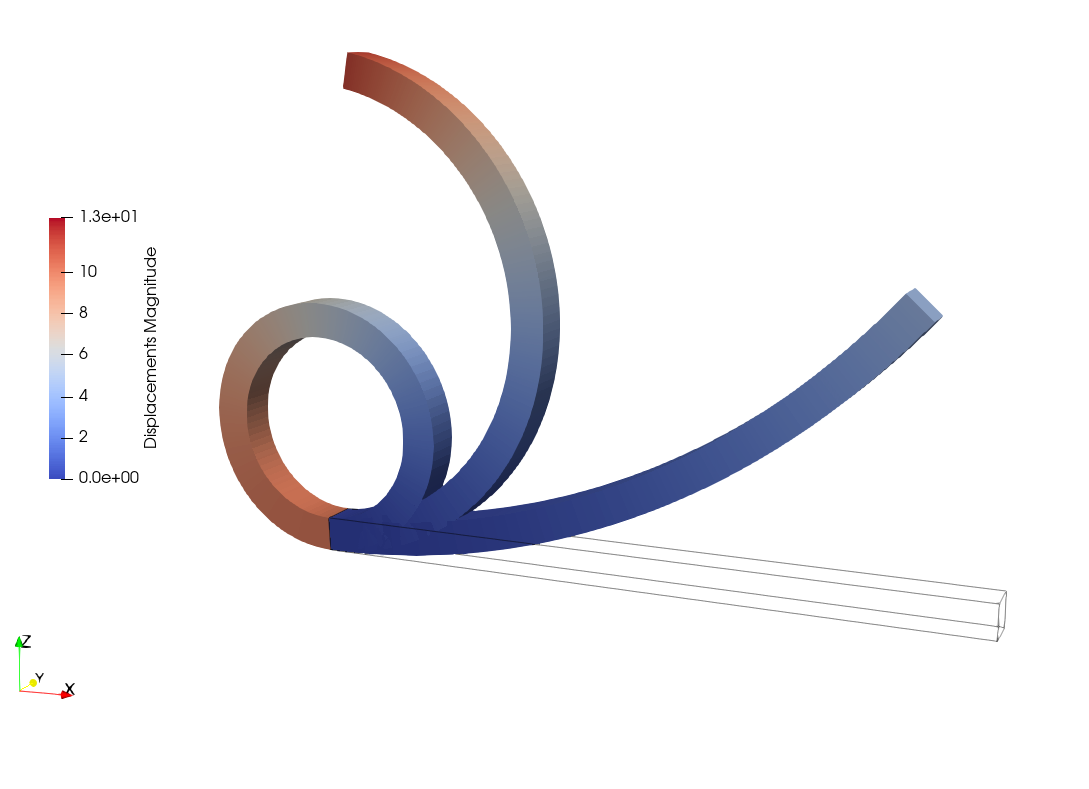
\includegraphics[width=0.46\textwidth]{./imagenes/ResultadosNumericos/uniformCantilever/Deformadas.png}}
		\subfigure[Valdiación para ángulo en el extremo.]
		{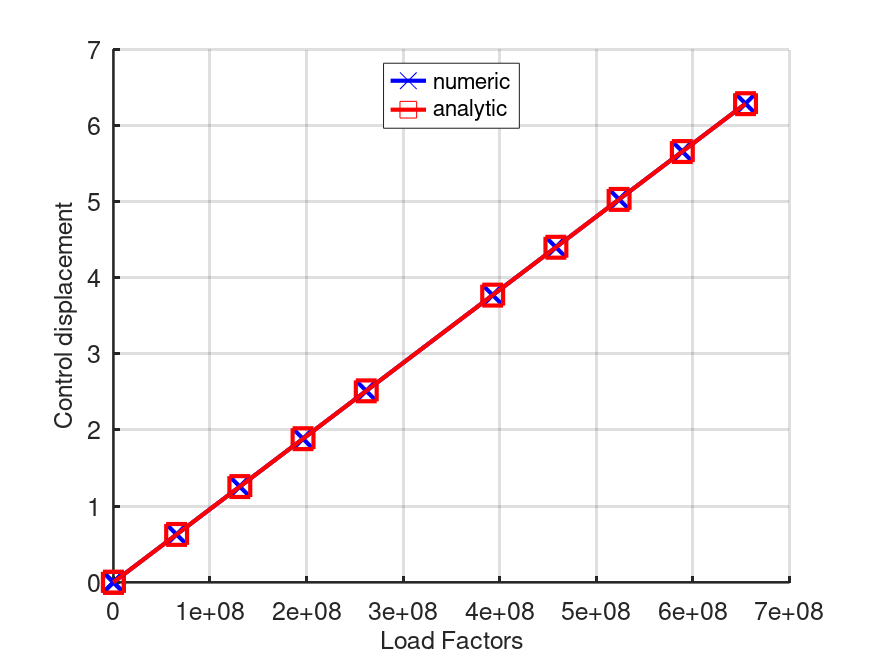
\includegraphics[width=0.46\textwidth]{./imagenes/ResultadosNumericos/uniformCantilever/uniformCantilever_analyticVerif.png}}
	\end{figure}
	
\end{frame}

%%%%%%%%%%%%%%%%%%%%%%%%%%%%%%%%%%%%%%%%%FRAME%%%%%%%%%%%%%%%%%%%%%%%%%%%%%%%%%%%%%%%%%
\begin{frame}{Sistemas de coordenadas corrotacional:}{}
	\begin{minipage}[t]{0.5\linewidth}
		\begin{figure}[htbp]
			\centering
			\def\svgwidth{60mm}
			\input{./imagenes/Preliminares/Corrotacional/IlusCorrotacional.pdf_tex}
			%	\caption{Descripción de las sistemas de coordenadas corrotacionales.}
		\end{figure}
	\end{minipage}\hfill
	\begin{minipage}[t]{0.5\linewidth}
		\begin{block}{Bases para cada configuración:}
			%	\begin{itemize}{Bases para cada configuración:}
			%		\item  Paramétrica: $(\bf{E_1},\bf{E_2},\bf{E_3})$
			%		\item  {\color{blue}Configuración de referencia} : $(\bf{r_1},\bf{r_2},\bf{r_3})$
			%		\item {\color{gray}Configuración de deformación rígida} : $(\bf{r_1},\bf{r_2},\bf{r_3})$
			%		\item  {\color{orange}Configuración deformada} :  $(\bf{t_1^i},\bf{t_2^i},\bf{t_3^i})$
			%	\end{itemize}
			Paramétrica: $(\bf{E_1},\bf{E_2},\bf{E_3})$\\
			{\color{blue}Configuración de referencia} : $(\bf{e_1},\bf{e_2},\bf{e_3})$\\
			{\color{gray}Configuración de deformación rígida} : $(\bf{r_1},\bf{r_2},\bf{r_3})$\\
			{\color{orange}Configuración deformada} :  $(\bf{t_1^i},\bf{t_2^i},\bf{t_3^i})$\\
		\end{block}
		\begin{block}{¿Cómo se vinculan las bases? :}
			Se definen las siguientes matrices de rotación...
		\end{block}
	\end{minipage}	
\end{frame}
%%%%%%%%%%%%%%%%%%%%%%%%%%%%%%%%%%%%%%%%FRAME%%%%%%%%%%%%%%%%%%%%%%%%%%%%%%%%%%%%%%%%%

\begin{frame}{Matrices de rotación:}{}
	\begin{minipage}[t]{0.5\linewidth}
		\begin{figure}[htbp]
			\centering
			\def\svgwidth{60mm}
			\input{./imagenes/Preliminares/Corrotacional/IlusCorrotacional2.pdf_tex}
		\end{figure}
	\end{minipage}\hfill
	\begin{minipage}[t]{0.5\linewidth}
		\begin{table}[htbp]
			\begin{tabular}{|c|c|}
				\hline
				Matriz & Vínculo de sistemas de referencia \\
				\hline \hline
				$\bf{R}_0$ &$(\bf{E_1},\bf{E_2},\bf{E_3})$ $\rightarrow$
				$(\bf{e_1},\bf{e_2},\bf{e_3})$   \\ \hline
				$\bf{R}_i^g$ & $(\bf{e_1},\bf{e_2},\bf{e_3})$ $\rightarrow$
				$(\bf{t_1^i},\bf{t_2^i},\bf{t_3^i})$ \\ \hline
				$\bf{\overline{R}}_i$ &
				$(\bf{r_1},\bf{r_2},\bf{r_3})$$\rightarrow$$(\bf{t_1^i},\bf{t_2^i},\bf{t_3^i})$
				\\ \hline
				$\bf{R}_r$ &
				$(\bf{t_1^i},\bf{t_2^i},\bf{t_3^i})$$\rightarrow$$(\bf{r_1},\bf{r_2},\bf{r_3})$ \\
				\hline
			\end{tabular}
			%		\caption{Caracterización de matrices en términos de los sistemas de referencia.}
		\end{table}
		\begin{block}{¿Como calcular $\bf{\overline{R}}_i$? }
			\begin{eqnarray}
			\bf{R_i^g}\bf{R_o}&=& \bf{R_r}\overline{\bf{R_i}}\\
			\bar{\bf{R_i}}&=&(\bf{R_r})^T\bf{R_i^g}\bf{R_o}
			\end{eqnarray}
		\end{block}
	\end{minipage}	
\end{frame}

%%%%%%%%%%%%%%%%%%%%%%%%%%%%%%%%%%%%%%%%%FRAME%%%%%%%%%%%%%%%%%%%%%%%%%%%%%%%%%%%%%%%%%
\begin{frame}[t]{Iteración corrotacional en ONSAS:}
	\begin{columns}[T,onlytextwidth]
		\begin{column}{.4\textwidth}
			\begin{minipage}{\textwidth}
				\vfill
				\begin{figure}
					\centering
					\def\svgwidth{60mm}
					\input{./imagenes/ResultadosNumericos/uniformCantilever/uniformCantileverBeamDisp.pdf_tex}
				\end{figure}
			\end{minipage}  
			
			\begin{minipage}{\textwidth}
				\begin{figure}
					\centering
					\def\svgwidth{60mm}
					\input{./imagenes/ResultadosNumericos/uniformCantilever/uniformCantileverBeamIters.pdf_tex}
				\end{figure}
			\end{minipage}
		\end{column}
		\begin{column}{.57\textwidth}
			\pause
			\begin{figure}[htbp]
				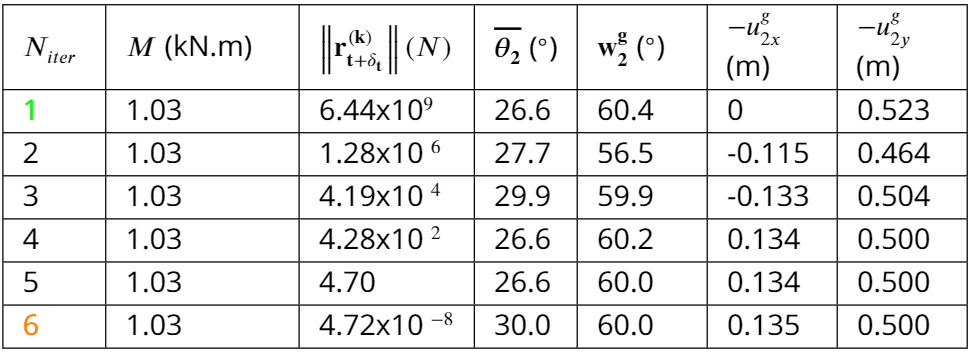
\includegraphics[width=1.01\textwidth]{./imagenes/ResultadosNumericos/uniformCantilever/TableIteraciones.png}
				\caption{Iteraciones en desplazamientos 1 elemento y $\Phi_f=$ 60 $^{\circ}$}	
			\end{figure}
		\end{column}
	\end{columns}
\end{frame}



%%%%%%%%%%%%%%%%%%%%%%%%%%%%%%%%%%%%%%%%FRAME%%%%%%%%%%%%%%%%%%%%%%%%%%%%%%%%%%%%%%%%%
\begin{frame}{Fuerza interna y matriz tangente:}
	\begin{minipage}[t]{0.46\linewidth}
		\begin{block}{Se definen los siguientes desplazamientos:}
			Locales: $~~\bf{d_l} = [\text{$\overline{u}$}, \boldsymbol{\overline{ \theta _1}^T},	\boldsymbol{ \overline{ \theta _2}^T}]^T$\\
			Globales: $\bf{ d_g} = [\bf{ u_1^g}^T, \bf{ u_2^g}^T, \bf{{w_1^g}^T}, \bf{{w_2^g}^T}]^T$
		\end{block}
		\begin{block}{La matriz $\bf{B}$ vincula sus variaciones :}
			En desplazamientos: $\bf{ d_l}=\bf{B}~\bf{ d_g}$ \\
			En Fuerzas: $\bf{f_{int}^g}=\bf{B}^T~\bf{ f_{int}^l}$
		\end{block}
	\end{minipage}\hfill
	\begin{minipage}[t]{0.49\linewidth}
	\begin{block}{Vector de fuerzas internas en coordenadas globales:}
		\begin{equation}
			\bf{f_{int}^g}=\bf{B}^T\bf{f_{int}^l}= \begin{bmatrix}
			\bf{r}\\
			\bf{PE^T}
			\end{bmatrix}\bf{f_{int}^l}
		\end{equation}
	\end{block}
	\begin{block}{Matriz tangente en coordenadas globales:}
		\begin{equation}
			\bf{K_g}=\bf{B}^T\bf{K_l}\bf{B}+\bf{D} f_{a1}-\bf{E}\bf{Q}\bf{G^T}\bf{E^T} +\bf{EGar}.
		\end{equation}
	\end{block}
	\end{minipage}
\end{frame}



%%%%%%%%%%%%%%%%%%%%%%%%%%%%%%%%%%%%%%%%%FRAME%%%%%%%%%%%%%%%%%%%%%%%%%%%%%%%%%%%%%%%%%
\begin{frame}{Fuerza inercial y matrices de masa tangentes:}
		\begin{minipage}[t]{0.45\linewidth}\vfill
			\begin{block}{Energía cinética y su variación para el elemento:}
				\begin{eqnarray}
					\textit{K}&=&\frac{1}{2}\int_{l_0} {\bf{v}}^T A_{\rho} {\bf{v}} + \boldsymbol{\omega}^T \bf{I_{\rho}} \boldsymbol{\omega}^T ~\text{$dl_0$}\\
					\delta\textit{K}&=&\bf{f_{ine}^T}~\delta\bf{d}_g
				\end{eqnarray}
			\end{block}
		\end{minipage}\hfill
		\begin{minipage}[t]{0.48\linewidth}
			\begin{block}{Vector de fuerzas inerciales en coordenadas globales:}
				\begin{equation}
				\bf{f}_{ine}= \int _{l_0} \left \{ \bf{H}_1^T\bf{R_r}^T \text{$A_\rho$}\bf{a} +\bf{H}_2^T \bf{R_r} [\bf{I}_\rho\boldsymbol{\alpha}+\widetilde{\boldsymbol{\omega}}\bf{I}_\rho\boldsymbol{\omega}] \right \} \text{$d_l$}
				\end{equation}
			\end{block}
			\begin{block}{Matrices dinámicas tangentes:}
				\begin{equation}
					\delta \bf{f_{ine}}= \bf{M} \delta {\bf{a}_g}+\bf{C}_k \delta {\bf{v}_g}+\bf{K}_k \delta \bf{d}_g
				\end{equation}
			\end{block}
		\end{minipage}
	\end{frame}
%%%%%%%%%%%%%%%%%%%%%%%%%%%%%%%%%%%%%%%     SECTION  %%%%%%%%%%%%%%%%%%%%%%%%%%%%%%%%%%%%%%%%%
\section[Metodología]{Metodología}

\AtBeginSection[]
{
	\ifnum \value{framenumber}>1
	\begin{frame}<beamer>
		\frametitle{Resultados}
		\tableofcontents[currentsection]
	\end{frame}
	\else
	\fi
}
%%%%%%%%%%%%%%%%%%SUBSECTION%%%%%%%%%%%%%%%%%%
\subsection[Modelado estructural]{Modelado estructural}

%%%%%%%%%%%%%%%%%%%%%%%%%%%%%%%%%%%%%%%%FRAME%%%%%%%%%%%%%%%%%%%%%%%%%%%%%%%%%%%%%%%%%
\begin{frame}{Modelado estructural de las líneas:}
		\begin{minipage}[t]{0.35\linewidth}
		\begin{figure}[htbp]
			\centering
			\def\svgwidth{50mm}
			\input{./imagenes/Metodologia/EsquemaInicial.pdf_tex}
%				\caption{Esquema del objeto de estudio.}
		\end{figure}
		\end{minipage}\hfill
		\begin{minipage}[t]{0.64\linewidth}
			\begin{block}{Hipótesis:}
				\begin{itemize}
				\item Los puntos A y D se encuentran a la misma altura.
				\pause
				\item No existe deslizamiento relativo entre las trenzas que conforman el conductor.
				\pause
				\item La condición inicial $\bf{u_0}$ es la solución estática al problema de peso propio.
				\pause
				\item Los aisladores se modelaron con elementos de barras de Green según {\color{blue} (Crisfield,1997) }.
				\pause
				\item No se incluyen las fuerzas de pretensado.
				\end{itemize}
			\end{block}
		\end{minipage}
\end{frame}
%%%%%%%%%%%%%%%%%%%SUBSECTION%%%%%%%%%%%%%%%%%%
\subsection[Modelado de viento]{Modelo de viento}
%%%%%%%%%%%%%%%%%%%%%%%%%%%%%%%%%%%%%%%%%FRAME%%%%%%%%%%%%%%%%%%%%%%%%%%%%%%%%%%%%%%%%%
\begin{frame}{Modelado de viento}
	\begin{minipage}[t]{0.48\linewidth}
		\begin{figure}[htbp]
			\centering
			\def\svgwidth{60mm}
			\input{./imagenes/Metodologia/VelRel.pdf_tex}
			\caption{Esquema en sistema de referencias relativo.}
		\end{figure}
	\end{minipage}\hfill
	\begin{minipage}[t]{0.48\linewidth}
		\vspace{-1.3cm}
		\begin{block}{Hipótesis de viento}
			\begin{itemize}
				\item Velocidad media predominante: $q,\bf{v_{y}},\bf{v_{z}}<<w_m$
				\item La velocidad incide perpendicular a la línea. 
				\item La fuerza \emph{lift} se desprecia frente al \emph{drag}.
			\end{itemize}
		\end{block}
		\pause
		\begin{block}{Fuerza de drag y velocidad relativa:}
			\begin{eqnarray}
					F_d &=& \frac{\rho d_c C_d}{2} V_{rel}^2\\
					\frac{V_{rel}^2}{w_m}&=&w_m + 2 (w_a-\bf{v}_{z}).\\
					F_d &=& \frac{\rho d_c C_d}{2} (w_m + 2 (w_a-\bf{v_{z}}))\text{$w_m$}
				\end{eqnarray}
		\end{block}
%			\begin{eqnarray}
%				\frac{V_{rel}^2}{w_m}&=&w_m + 2 (w_a-\bf{v_{z}).\\
%				F_z= &=& \frac{\rho d_c C_d}{2} (u_m^2+w_a^2-2 w_m \text{$\bf{v_{z}$})\cos(\beta_r)=...\\
%				...&=&F_d=\bar{F_z}+F_a-F_{vis}
%			\end{eqnarray}
	\end{minipage}
\end{frame}
%%%%%%%%%%%%%%%%%%%%%%%%%%%%%%%%%%%%%%%%%FRAME%%%%%%%%%%%%%%%%%%%%%%%%%%%%%%%%%%%%%%%%%
\begin{frame}{Modelado de viento}
	\begin{minipage}[t]{0.48\linewidth}
		\begin{figure}[htbp]
			\centering
			\def\svgwidth{60mm}
			\input{./imagenes/Metodologia/VelRel.pdf_tex}
			\caption{Esquema en sistema de referencias relativo.}
		\end{figure}
	\end{minipage}\hfill
	\begin{minipage}[t]{0.48\linewidth}
		\vspace{-1.3cm}
		\begin{block}{Ángulo relativo:}
			\begin{eqnarray}
				\tan (\beta_r) &=& \frac{q-\bf{v_y}}{w_m - \bf{v}_{z} + \text{$w_a$}} \approx 0 \\
			F_z &=& F_d \cos(\beta_r)=\bar{F_z}+F_{za}-F_{vis}
			\end{eqnarray}
		\end{block}
		\begin{block}{Desglose de fuerzas}
				\begin{eqnarray}
					\bar{F_z} &=&  \frac{\rho d_c C_d}{2} (w_m^2)\\
					F_{za} &=&  \frac{\rho d_c C_d}{2} (w_a^2)\approx 0\\
					F_{vis}  &=& \frac{\rho d_c C_d}{2} (2 \text{$\bf{v_{z}}$} w_m)
				\end{eqnarray}  
		\end{block}
	\end{minipage}
\end{frame}
%%%%%%%%%%%%%%%%%%%%%%%%%%%%%%%%%%%%%%%%%%%FRAME%%%%%%%%%%%%%%%%%%%%%%%%%%%%%%%%%%%%%%%%%
%%%%%%%%%%%%%%%%%%%%%%%%%%%%%%%%%%%%%%%%%     SECTION  %%%%%%%%%%%%%%%%%%%%%%%%%%%%%%%%%%%%%%%%%
 \section[Resultados Numéricos]{Resultados Numéricos}
\subsection[Viga en voladizo con ángulo recto]{Viga en voladizo con ángulo recto}
%%%%%%%%%%%%%%%%%%%%%%%%%%%%%%%%%%%%%%%%%%FRAME%%%%%%%%%%%%%%%%%%%%%%%%%%%%%%%%%%%%%%%%%
\begin{frame}[t]{Viga en voladizo con ángulo recto:}
	\begin{columns}[T,onlytextwidth]
		\begin{column}{.58\textwidth}
			\begin{minipage}{\textwidth}
				\begin{figure}[htbp]
				\subfigure[Vista frontal ]{	\def\svgwidth{30mm}
				\input{./imagenes/ResultadosNumericos/RightAngeCantilever/Ilustracion2Dxy.pdf_tex}}\label{fig:RN:RA:Ilusxy}
				\subfigure[Vista lateral ]{	\def\svgwidth{20mm}
				\input{./imagenes/ResultadosNumericos/RightAngeCantilever/Ilustracion2Dyz.pdf_tex}}\label{fig:RN:RA:Ilusyz}
%				\caption{Disposición geométrica de la estructura.} 	\label{fig:RN:RA:esquemas}
				\end{figure}
					\begin{figure}[htbp]
					
					\def\svgwidth{35mm}
					\input{./imagenes/ResultadosNumericos/RightAngeCantilever/FuerzaZ.pdf_tex}
%					\caption{Perfil de fuerza $F_z$}
				\end{figure}
		\end{minipage}  
		\end{column}
		\begin{column}{.4\textwidth}
			\begin{onlyenv}<2->
				\begin{minipage}{\textwidth}
					\vspace{-1cm}
					\begin{block}{Propiedades y dimensiones:}
						\begin{itemize}
							\item $GA= EA=10^6$ y $GJ = EI =10^3$.  
							\item $L=10$.
						\end{itemize}	 
					\end{block}
				\end{minipage}
			\end{onlyenv}
			\begin{onlyenv}<3->
				\begin{minipage}{\textwidth}
					\begin{block}{Parámetros computacionales:}
						\begin{itemize}
							\item 10 elementos por barra.
							\item Parámetro de HHT: $\alpha_{HHT}=-0.05$
							\item $t_f=20$ s y $\delta_t =-0.25$ s .
							\item $tol_u =1x10^{-5} $ $tol_r =1$$x10^{-7} $  
						\end{itemize}	 
					\end{block}
				\end{minipage}
			\end{onlyenv}
		\end{column}
	\end{columns}
\end{frame}
%%%%%%%%%%%%%%%%%%%%%%%%%%%%%%%%%%%%%%%%%FRAME%%%%%%%%%%%%%%%%%%%%%%%%%%%%%%%%%%%%%%%%%
\begin{frame}{Viga en voladizo con ángulo recto:}
	\begin{figure}[htbp]
		\centering
		\def\svgwidth{80mm}
		\input{./imagenes/ResultadosNumericos/RightAngeCantilever/Deformadas.pdf_tex}
%		\caption{Estructura deformada en los instantes $4$ s, $11$ s y $21$ s.}
	\end{figure}
\end{frame}
%%%%%%%%%%%%%%%%%%%%%%%%%%%%%%%%%%%%%%%%%FRAME%%%%%%%%%%%%%%%%%%%%%%%%%%%%%%%%%%%%%%%%%
\begin{frame}{Validación nodo A:}
		\vspace{-0.1cm}
\begin{figure}[htbp]
	\centering
	\subfigure[Desplazamiento vertical de A según $y$]{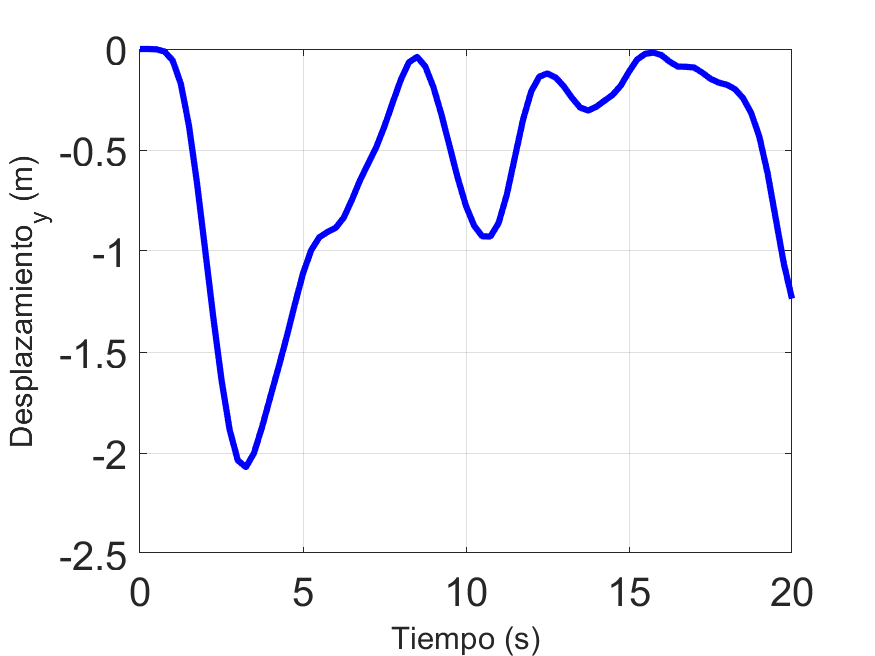
\includegraphics[width=0.48\textwidth]{./imagenes/ResultadosNumericos/RightAngeCantilever/RA_Dispy_NodeA.png}}
	\subfigure[Desplazamiento vertical de A según $y$ por {\color{blue}(Le,2014)} ] {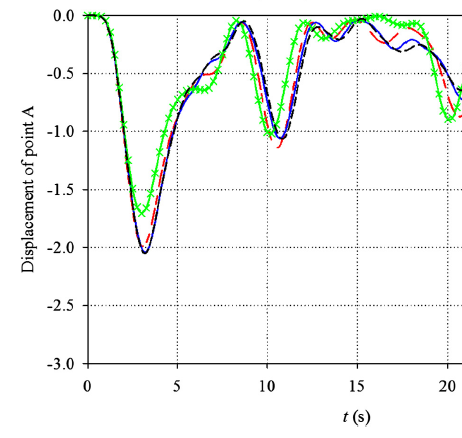
\includegraphics[width=0.37\textwidth]{./imagenes/ResultadosNumericos/RightAngeCantilever/BattiniDispA.png}}
	\caption{Comparación desplazamientos del nodo {\color{blue} A}.}
\end{figure}
\end{frame}
%%%%%%%%%%%%%%%%%%%%%%%%%%%%%%%%%%%%%%%%%  FRAME  %%%%%%%%%%%%%%%%%%%%%%%%%%%%%%%%%%%%%%%%%
\begin{frame}{Validación del nodo B:}
	\vspace{-0.1cm}
	\begin{figure}[htbp]
		\centering
		\subfigure[Desplazamiento vertical de B según $z$ ]{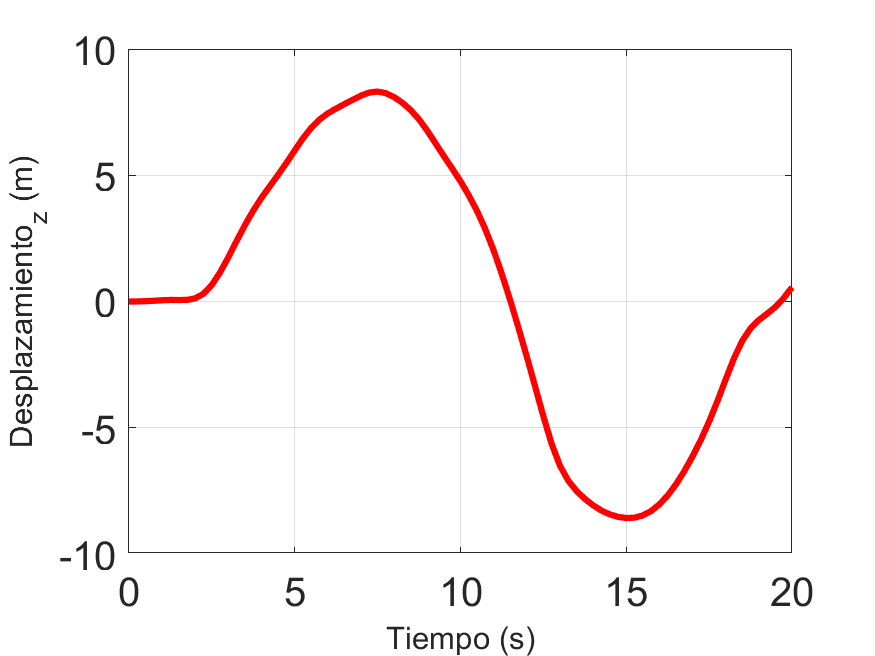
\includegraphics[width=0.48\textwidth]{./imagenes/ResultadosNumericos/RightAngeCantilever/RA_Dispz_NodeB.png}}
		\subfigure[Desplazamiento transversal según $z$ por {\color{blue}(Le,2014)} ] {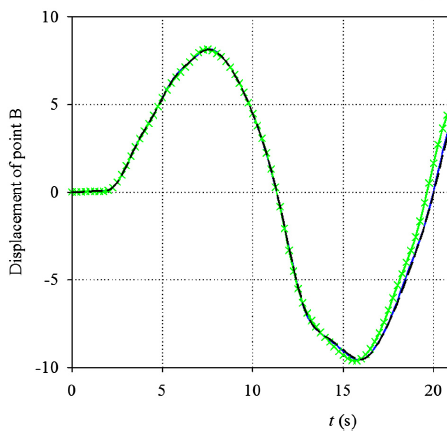
\includegraphics[width=0.37\textwidth]{./imagenes/ResultadosNumericos/RightAngeCantilever/BattiniDispB.png}}
		\caption{Comparación desplazamientos del nodo B.} \label{fig:RN:RA:DispsA}
	\end{figure}
\end{frame}

%%%%%%%%%%%%%%%%%%%%%%%%%%%%%%%%%%%%%%%%%%  FRAME  %%%%%%%%%%%%%%%%%%%%%%%%%%%%%%%%%%%%%%%%%
\subsection[Modelo simplificado de una línea]{Modelo simplificado de una línea}
%%%%%%%%%%%%%%%%%%%%%%%%%%%%%%%%%%%%%%%%%FRAME%%%%%%%%%%%%%%%%%%%%%%%%%%%%%%%%%%%%%%%%%
\begin{frame}[t]{Modelo simplificado de una línea:}
	\begin{columns}[T,onlytextwidth]
		\begin{column}{.58\textwidth}
			\begin{minipage}{\textwidth}
					\begin{figure}[htbp]
					\centering
					\subfigure[Vista en perspectiva ]{	\def\svgwidth{40mm}
						\input{./imagenes/ResultadosNumericos/SimpleCable/EsquemaCable.pdf_tex}}
					\subfigure[Sección transversal ]{	\def\svgwidth{40mm}
						\input{./imagenes/ResultadosNumericos/SimpleCable/PerfilCable.pdf_tex}}
					\caption{Disposición geométrica de la línea.} 
				\end{figure}
			\end{minipage}  
		\end{column}
		\begin{column}{.4\textwidth}
			\begin{onlyenv}<2->
				\begin{minipage}{\textwidth}
					\vspace{-1.7cm}
					\begin{block}{Propiedades y dimensiones:}
						\begin{itemize}
							\item Conductor ASCR 7/26
							\item $L_c = 267$ m y $d_c = 2.81$ cm
							\item $m   = 1.8 $ kg/m
							\item $EA  = 29700$ kN
							\item $EI  = 2100 $ (N.m$^2$) $GJ  = 159$ (N.m$^2$)
						\end{itemize}	 
					\end{block}
				\end{minipage}
			\end{onlyenv}
		\begin{onlyenv}<3->
			\begin{minipage}{\textwidth}
				\begin{block}{Parámetros computacionales:}
					\begin{itemize}
						\item $\alpha_{HHT} = -0.1$
						\item 150 elementos de cable. 
						\item $tf= 350$ y $\delta_t = 1$ s
						\item $tol_u =1$$x10^{-5} $ $tol_r =1x10^{-7} $   
					\end{itemize}	 
				\end{block}
			\end{minipage}
		\end{onlyenv}
		\end{column}
	\end{columns}
\end{frame}
%%%%%%%%%%%%%%%%%%%%%%%%%%%%%%%%%%%%%%%%%FRAME%%%%%%%%%%%%%%%%%%%%%%%%%%%%%%%%%%%%%%%%%

\begin{frame}{Acción del viento:}
	\begin{figure}[htbp]
		\centering
		\subfigure[Perfil de velocidad en $z$]{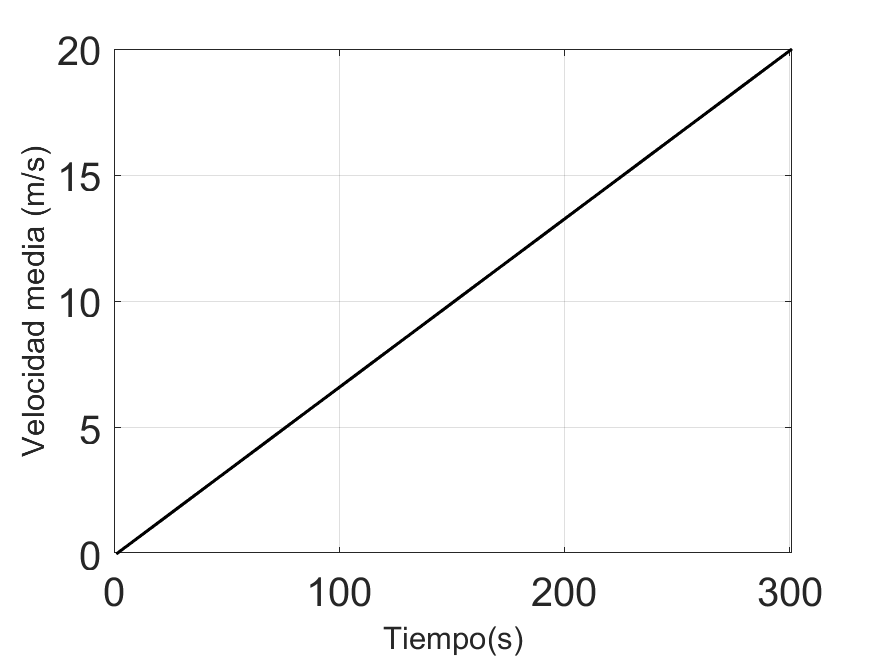
\includegraphics[width=0.42\textwidth]{./imagenes/ResultadosNumericos/SimpleCable/PerfilVm_TL_Foti.png}}
		\subfigure[Perfil de fuerza en $z$] {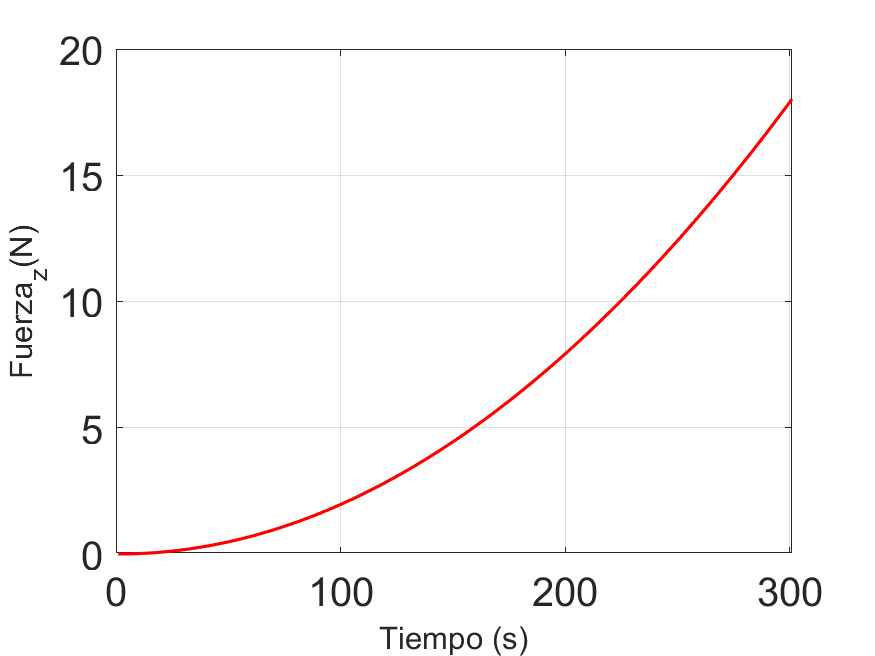
\includegraphics[width=0.42\textwidth]{./imagenes/ResultadosNumericos/SimpleCable/FuerzaNodalZ_TLFoti.png}}		
		\caption{Perfil de viento aplicado en $z$.}
	\end{figure}
\end{frame}

%%%%%%%%%%%%%%%%%%%%%%%%%%%%%%%%%%%%%%%%%FRAME%%%%%%%%%%%%%%%%%%%%%%%%%%%%%%%%%%%%%%%%%

\begin{frame}{Ángulo de balanceo:}
	\begin{figure}[htbp]
		\centering
		\subfigure[Esquema del ángulo de control $\Phi$.]{	\def\svgwidth{50mm}\input{./imagenes/ResultadosNumericos/SimpleCable/AnguloCable.pdf_tex}}
		\subfigure[Ángulo de balanceo $\Phi$ en función de la velocidad media $W(t)$.] {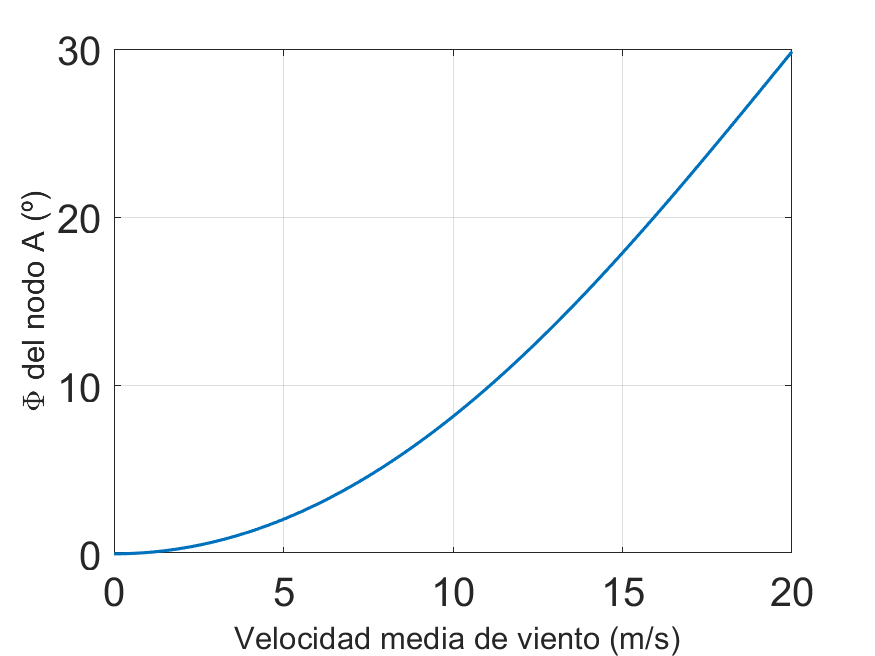
\includegraphics[width=0.42\textwidth]{./imagenes/ResultadosNumericos/SimpleCable/Angulo_Foti.png}}
	\end{figure}
\end{frame}
\subsection[Viga en voladizo con péndulo]{Viga en voladizo con péndulo}
%%%%%%%%%%%%%%%%%%%%%%%%%%%%%%%%%%%%%%%%%FRAME%%%%%%%%%%%%%%%%%%%%%%%%%%%%%%%%%%%%%%%%%
\begin{frame}[t]{Viga en voladizo con péndulo:}
	\begin{columns}[T,onlytextwidth]
		\begin{column}{.58\textwidth}
			\begin{minipage}{\textwidth}
				\begin{figure}[htbp]
					\centering
					\def\svgwidth{70mm}
					\input{./imagenes/ResultadosNumericos/CantieleverPendulum/cantieleverPendulum.pdf_tex}
				\end{figure}
			\end{minipage}  
		\end{column}
		\begin{column}{.4\textwidth}
			\begin{onlyenv}<2->
				\begin{minipage}{\textwidth}
					\vspace{-1cm}
					\begin{block}{Propiedades y dimensiones:}
						\begin{itemize}
							\item {\color{blue} Truss (T)}: $L= 3.04$ m $EA_t= 100$ GN $\nu_T=.3$ $\rho_T=65.7$ kg/m $^3$.
							\item {\color{red} Beam (B)}:  $EA_b= 2.33$ MN $EI= 18.5$ kN.m$^2$   $\rho_B=65.7$ kg/m$^3$
						\end{itemize}	 
					\end{block}
				\end{minipage}
			\end{onlyenv}
			\begin{onlyenv}<3->
				\begin{minipage}{\textwidth}
					\begin{block}{Parámetros computacionales:}
						\begin{itemize}
							\item $\alpha_{HHT} = -0.01$
							\item 1 elementos de barra y 10  de viga. 
							\item $tol_u =1$$x10^{-5} $ $tol_r =1x10^{-7} $ 
						\end{itemize}	 
					\end{block}
				\end{minipage}
			\end{onlyenv}
		\end{column}
	\end{columns}
\end{frame}


%%%%%%%%%%%%%%%%%%%%%%%%%%%%%%%%%%%%%%%%%%FRAME%%%%%%%%%%%%%%%%%%%%%%%%%%%%%%%%%%%%%%%%%
\subsection[Sistema de transmisión]{Sistema de transmisión}
%%%%%%%%%%%%%%%%%%%%%%%%%%%%%%%%%%%%%%%%%%FRAME%%%%%%%%%%%%%%%%%%%%%%%%%%%%%%%%%%%%%%%%%
\begin{frame}[t]{Sistema de transmisión:}
	\begin{columns}[T,onlytextwidth]
		\begin{column}{.58\textwidth}
			\begin{minipage}{\textwidth}
				\begin{figure}[htbp]
					\centering
					\def\svgwidth{70mm}
					\input{./imagenes/ResultadosNumericos/TransmissionTormenta/IlustracionTormenta.pdf_tex}
				\end{figure}
			\end{minipage}  
		\end{column}
		\begin{column}{.4\textwidth}
			\begin{onlyenv}<2->
				\begin{minipage}{\textwidth}
					\vspace{-1cm}
					\begin{block}{Propiedades y dimensiones:}
						\begin{itemize}
							\item {\color{gray} Conductor ASCR 7/26  }:$EA_b= 2.33$ MN $EI= 18.5$ kN.m$^2$   $\rho_B=65.7$ kg/m$^3$.
							\item {\color{red} ASTM A572 laminado en caliente}:  $E= 300$ GPa $D_c= 14$ m  $L_1= 26$ m $L_2= 31$ m y $L_3= 39$ m  
						\end{itemize}	 
					\end{block}
				\end{minipage}
			\end{onlyenv}
			\begin{onlyenv}<3->
				\begin{minipage}{\textwidth}
					\begin{block}{Parámetros computacionales:}
						\begin{itemize}
							\item $\alpha_{HHT} = -0.01$
							\item 663 elementos de barra y 150 elementos por cable. 
							\item $tol_u =1$$x10^{-5} $ $tol_r =1x10^{-5} $   
						\end{itemize}	 
					\end{block}
				\end{minipage}
			\end{onlyenv}
		\end{column}
	\end{columns}
\end{frame}
%Poner Color a la carga distribuída 
%%%%%%%%%%%%%%%%%%%%%%%%%%%%%%%%%%%%%%%%%%FRAME%%%%%%%%%%%%%%%%%%%%%%%%%%%%%%%%%%%%%%%%%
\begin{frame}{Acción del viento:}
	\begin{figure}[htbp]
		\centering
		\subfigure[Perfil de vlocidad de viento en $z$ ] {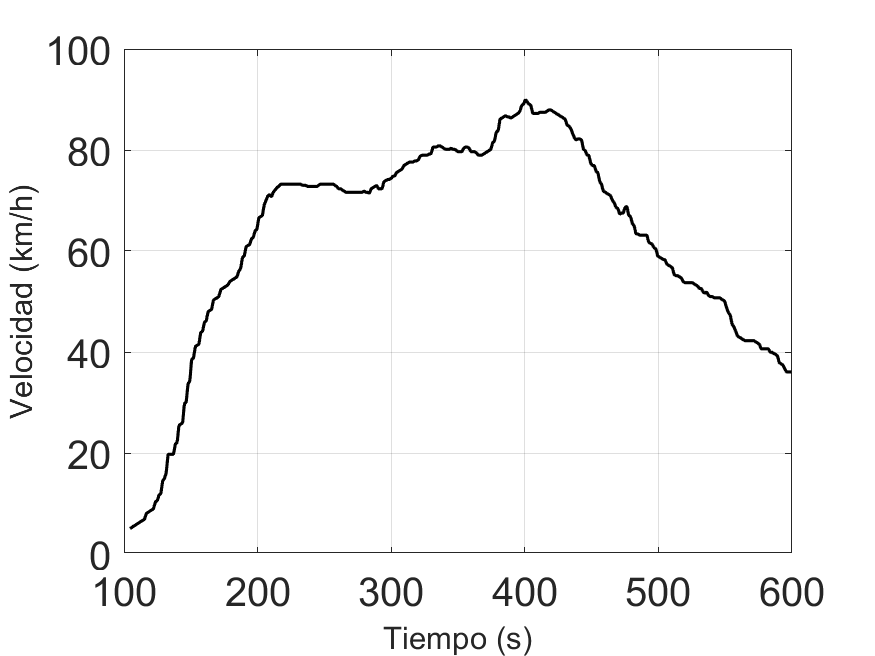
\includegraphics[width=0.42\textwidth]{./imagenes/ResultadosNumericos/TransmissionTormenta/VelocidadNodalX_TS.png}}
		\subfigure[Carga aplicada sobre los nodos]{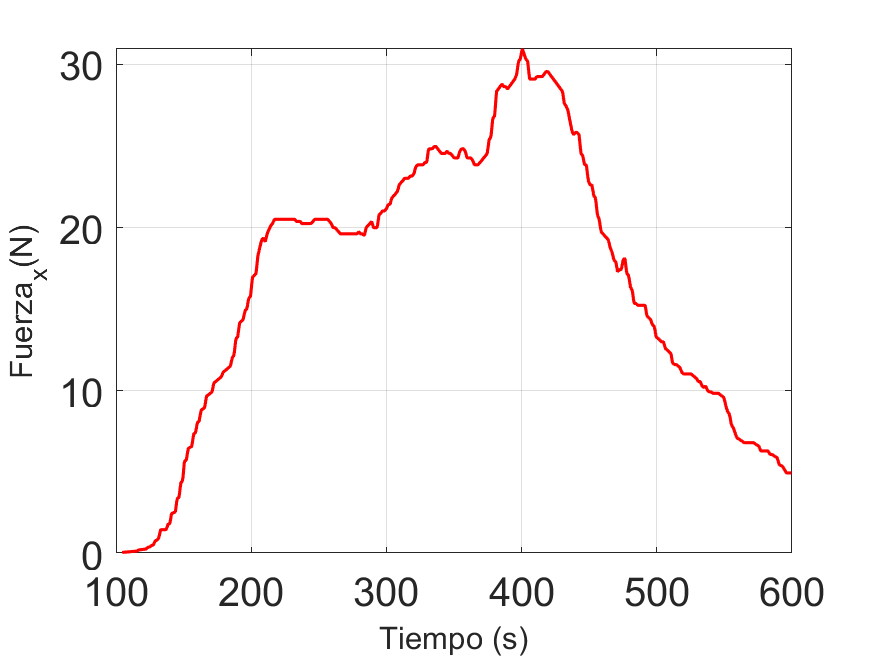
\includegraphics[width=0.42\textwidth]{./imagenes/ResultadosNumericos/TransmissionTormenta/FuerzaNodalX_TS.png}}
		\caption{Perfil de viento aplicado en $z$ según \color{blue}(Stengel,2017).}
	\end{figure}
\end{frame}
%%%%%%%%%%%%%%%%%%%%%%%%%%%%%%%%%%%%%%%%%%FRAME%%%%%%%%%%%%%%%%%%%%%%%%%%%%%%%%%%%%%%%%%
\begin{frame}{Resultados ángulo de balanceo:}
	\begin{figure}[htbp]
		\centering
		\subfigure[Ilustración del ángulo de balanceo $\Phi$]{	\def\svgwidth{50mm} 			\input{./imagenes/ResultadosNumericos/TransmissionTormenta/IlustracionAngulo.pdf_tex}}
		\subfigure[Perfil de velocidades en $z$ según \color{blue}(Stengel,2017)] {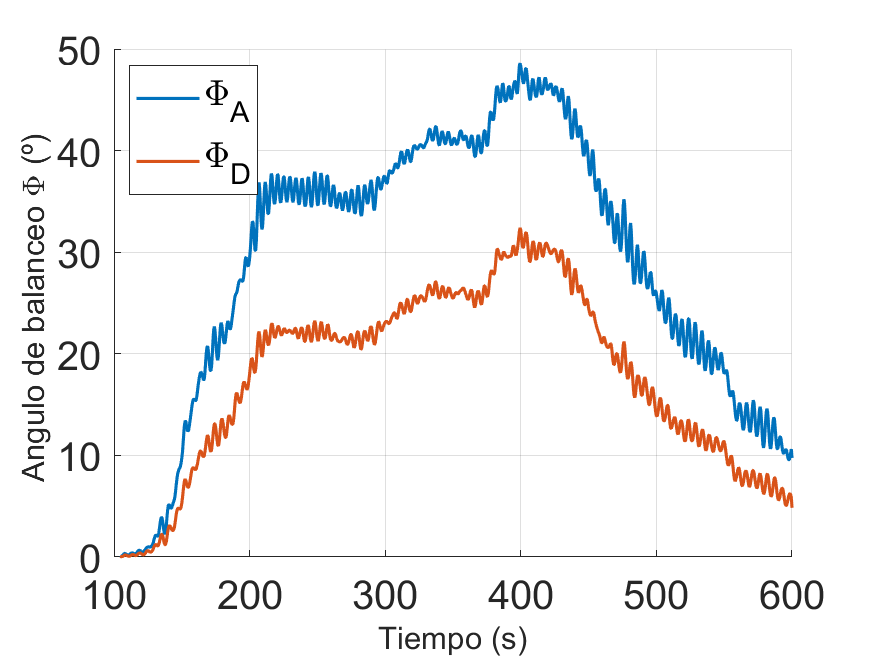
\includegraphics[width=0.42\textwidth]{./imagenes/ResultadosNumericos/TransmissionTormenta/Angulo_TS_NodeAD.png}}
		\caption{Ángulos de balanceo en cadenas aisladoras.}
	\end{figure}
\end{frame}

%%%%%%%%%%%%%%%%%%%%%%%%%%%%%%%%%%%%%%%%%%%%%%%%FRAM%%%%%%%%%%%%%%%%%%%%%%%%%%%%%

\begin{frame}{Resultados desplazamientos nodales:}
	\begin{figure}[htbp]
		\centering
		\subfigure[Desplazamientos en $x$ nodos B y C. ]{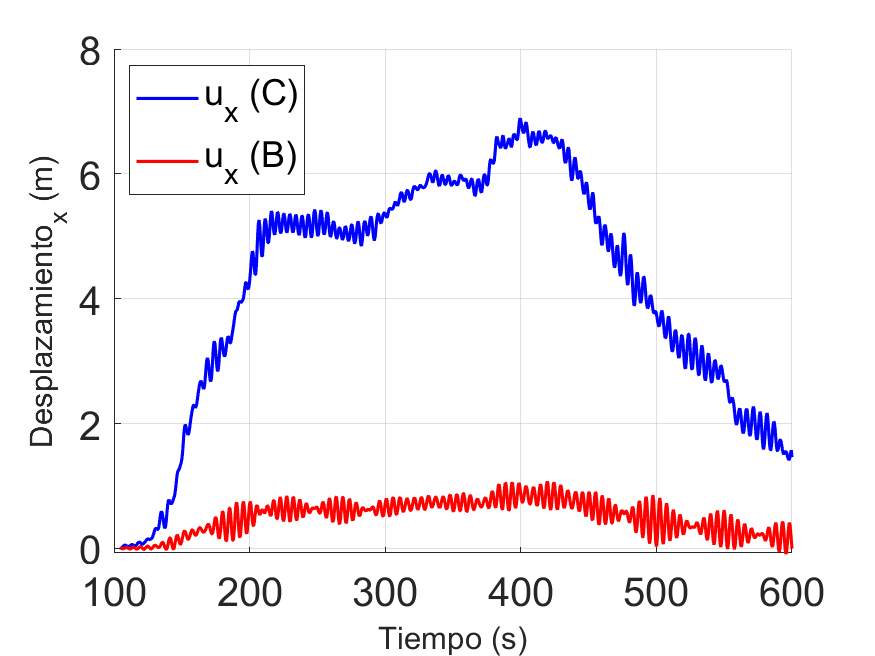
\includegraphics[width=0.48\textwidth]{./imagenes/ResultadosNumericos/TransmissionTormenta/DispXTS_NodeCB.png}\label{fig:RN:Transmission:DispXCB}}
		\subfigure[Desplazamientos en $z$ nodo B y C.] {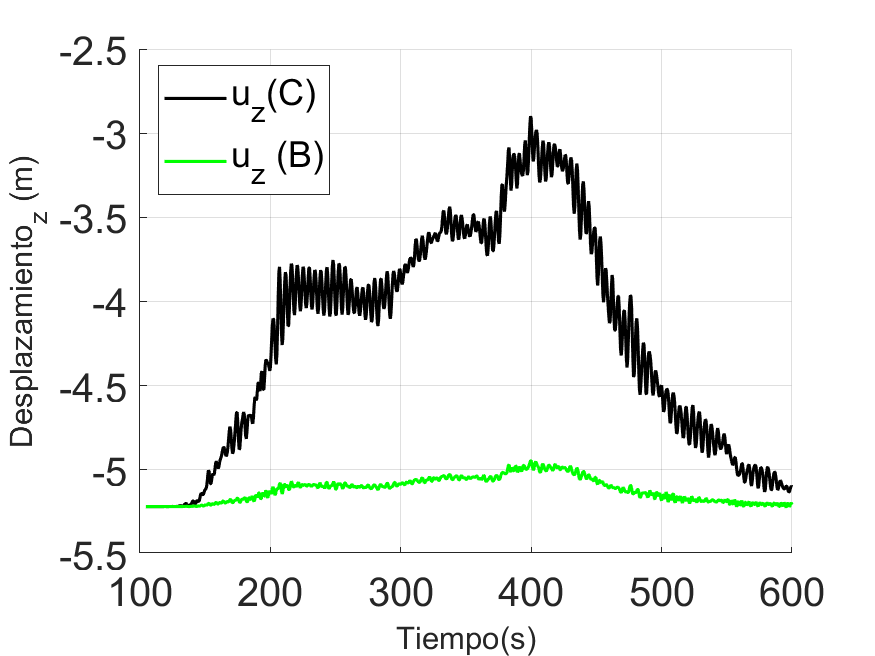
\includegraphics[width=0.48\textwidth]{./imagenes/ResultadosNumericos/TransmissionTormenta/DispZTS_NodeCB.png}\label{fig:RN:Transmission:DispZCB}}
		\caption{Desplazamientos de los nodos medios B y C. \label{fig:RN:Transmission:DispsCB}}
	\end{figure}
\end{frame}
%%%%%%%%%%%%%%%%%%%%%%%%%%%%%%%%%%%%%%%%     SECTION  %%%%%%%%%%%%%%%%%%%%%%%%%%%%%%%%%%%%%%%%%
\section[Conclusiones]{Conclusiones}

\AtBeginSection[]
{
	\ifnum \value{framenumber}>1
	\begin{frame}<beamer>
		\frametitle{}
		\tableofcontents[currentsection]
	\end{frame}
	\else
	\fi
}
%%%%%%%%%%%%%%%%%%%%%%%%%%%%%%%%%%%%%%%%%%FRAME%%%%%%%%%%%%%%%%%%%%%%%%%%%%%%%%%%%%%%%%%
\begin{frame}{Conclusiones }
	\begin{itemize}
		\item  Se implementó y validó dentro del código abierto \href{https://github.com/ONSAS/ONSAS.m/}{ONSAS} una formulación corrotacional de vigas 3D para la simulación de problemas dinámicos no lineales de estructuras tridimensionales formadas por vigas.
		\pause 
		\item Se extendió analíticamente la formulación corrotacional para elementos de cables incorporando términos de amortiguamiento aerodinámicos.
		\pause
		\item Se generó un modelo que representa el acoplamiento entre torres y conductores sometido a la acción de un perfil tipo CC.
		\pause
		\item Según los resultados del modelo, las tormentas convectivas afectan a las líneas generando desplazamientos de casi 7 metros y ángulos de hasta 40$^{\circ}$ en la cadena aisladora. 
	\end{itemize}
\end{frame}
%%%%%%%%%%%%%%%%%%%%%%%%%%%%%%%%%%%%%%%%%%FRAME%%%%%%%%%%%%%%%%%%%%%%%%%%%%%%%%%%%%%%%%%
\begin{frame}{Trabajos a futuro }
	\begin{itemize}
		\item Verificar la hipótesis de no deslizamiento en las lingas que conforman el conductor según {\color{blue}(Foti,2017)}.
		\pause
		\item Obtener resultados experimentales específicos sobre líneas de alta tensión que permitan validar el modelo. 
		\pause
		\item Modelar las principales líneas de trasmisión afectados por tormentas severas colaborativamente con la empresa UTE.
		\pause
		\item Incluir perfiles de velocidades capturados por estaciones meteorológicas en Uruguay e integrar esta investigación con los avances en Ingeniería del Viento del grupo de Eolo Dinámica del IMFIA . 
		\pause 
		\item  Escudriñar  las oscilaciones de alta frecuencia observadas en los resultados numéricos del ejemplo de trasmisión eléctrica.
		\pause 
		\item Incluir en el análisis teórico de la formulación corrotacional condiciones de Dirichlet no homogéneas en desplazamientos para el modelado del pretensado.
	\end{itemize}
\end{frame}
%%%%%%%%%%%%%%%%%%%%%%%%%%%%%%%%%%%%%%%%%%FRAME%%%%%%%%%%%%%%%%%%%%%%%%%%%%%%%%%%%%%%%%%
\begin{frame}[t]{Animación:}
	\begin{columns}[T,onlytextwidth]
		\begin{column}{.58\textwidth}
			\begin{minipage}{\textwidth}
				\vspace{-.5cm}
				\begin{figure}[htbp]
					\centering
				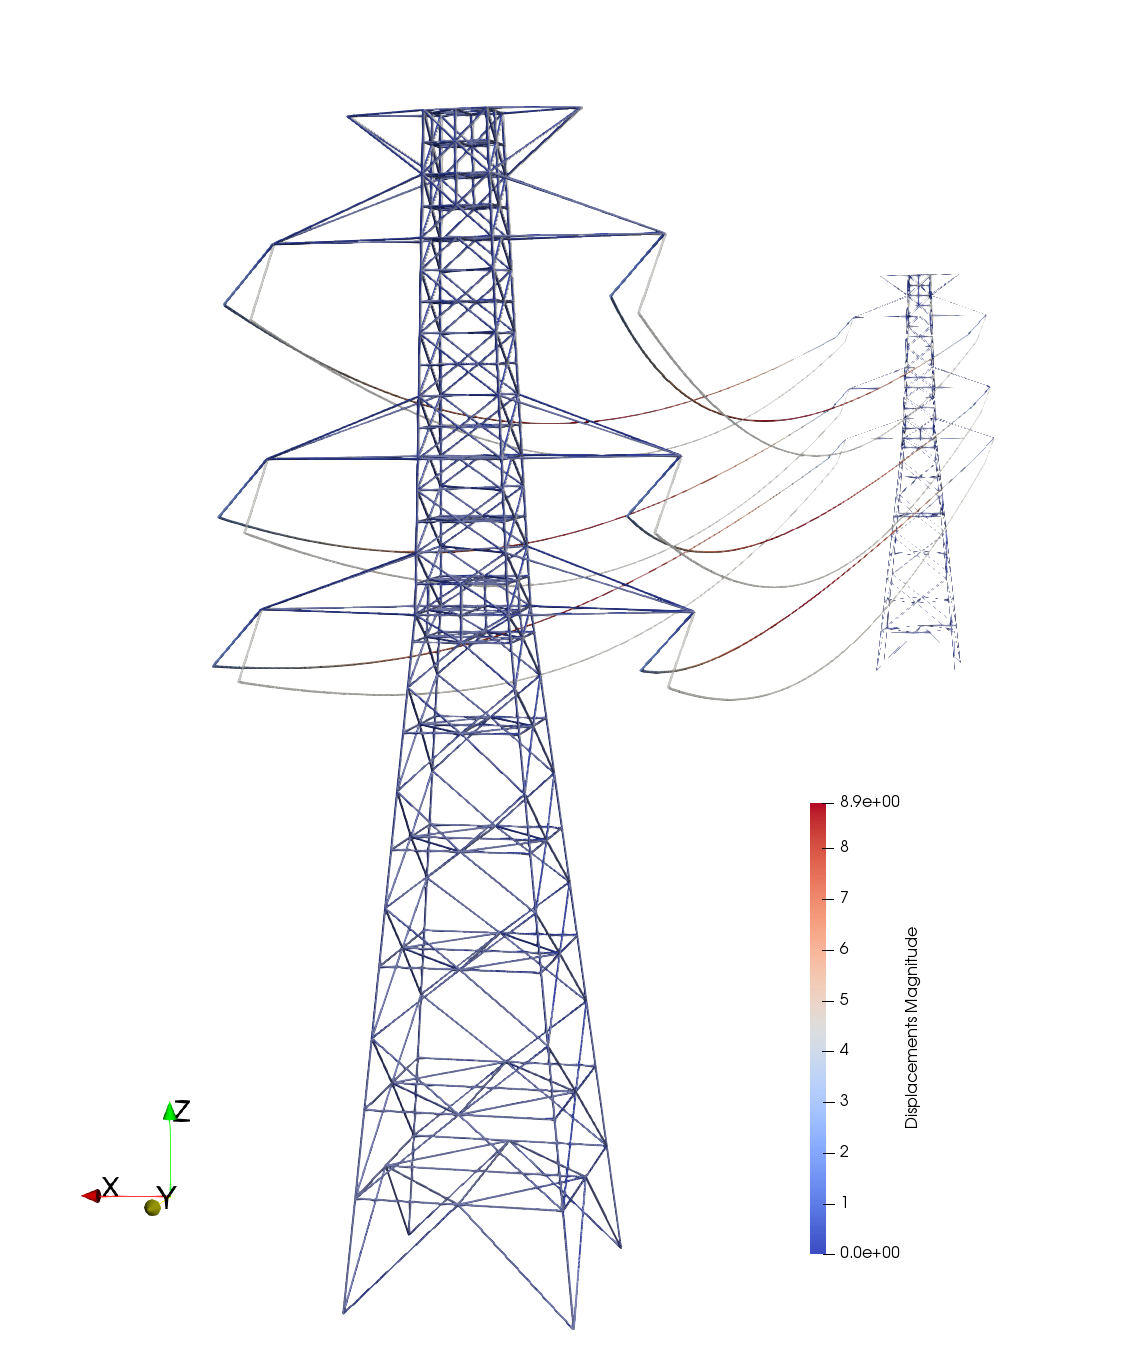
\includegraphics[width=0.6\textwidth]{./imagenes/ResultadosNumericos/TransmissionTormenta/Perspectiva.png}
				\end{figure}
			\end{minipage}  
		\end{column}
		\begin{column}{.4\textwidth}
			\begin{onlyenv}<2->
				\begin{minipage}{\textwidth}
					\begin{block}{Animación...}
						Ejemplo de dos torres con la fuerza aplicada en todos los puntos. 
					\end{block}
				\end{minipage}
			\end{onlyenv}
		\end{column}
	\end{columns}
\end{frame}

%%%%%%%%%%%%%%%%%%%%%%%%%%%%%%%%%%%%%%%%%%FRAME%%%%%%%%%%%%%%%%%%%%%%%%%%%%%%%%%%%%%%%%%
\begin{frame}[t]{Gracias:}
	\begin{alertblock}{Gracias...}
		¡!
	\end{alertblock}
\pause
\begin{alertblock}{¿Preguntas?}
	¿? 
\end{alertblock}
\end{frame}
%%%%%%%%%%%%%%%%%%%%%%%%%%%%%%%%%%%%%%%%%%FRAME%%%%%%%%%%%%%%%%%%%%%%%%%%%%%%%%%%%%%%%%%
\begin{frame}{Referencias principales:}
	\begin{itemize}
		\item {\color{blue}(Le,2014)}: Le, T. N., Battini, J. M. y Hjiaj, M. (2014). A consistent 3D corotational beam element for nonlinear dynamic analysis of exible structures. Computer Methods in Applied Mechanics and Engineering, 269, 538-565.
		\item {\color{blue}(Viera,1969)} : Vieira, S.E., 1969. Tiempo y Clima, ed. nuestra tierra, vol. 8, 68pp.
		\item {\color{blue}(Li,2000)}: Li, C.Q., 2000. A stochastic model of severe thunderstorms for transmission line design. Probabilist. Eng. Mech. 15 (4), 359–364.
		\item{\color{blue}(Crisfield,1997)} Crisfield, M. A. (1997). Non-linear finite element analysis of solids and structures, Vol. 2. John Wiley and Sons.
		\item{\color{blue}(Simo y  Vu-Quoc ,1988) }Simo, J. C. y Vu-Quoc, L. (1988). On the dynamics in space of rods undergoing large motions and geometrically exact approach. Computer methods in applied mechanics and engineering, 66 (2), 125-161.
	\end{itemize}
\end{frame}

%%%%%%%%%%%%%%%%%%%%%%%%%%%%%%%%%%%%%%%%%FRAME%%%%%%%%%%%%%%%%%%%%%%%%%%%%%%%%%%%%%%%%%

\begin{frame}{Referencias principales:}
	\begin{itemize}
		\item {\color{blue}(Durañona,2019)}: Durañona, V., Marchesoni, E. y Salles, R. (2019). A first characterization of high winds that afect the energy distribution system of Uruguay and their related facts. Journal of Wind Engineering and Industrial Aerodynamics, 128-138.
		\item{\color{blue}(Stengel,2017)} Stengel, D. y Thiele, K. (2017). Measurements of downburst wind loading acting on an overhead transmission line in Northern Germany. Procedia engineering, 199, 3152-3157.
 		\item {\color{blue}(Foti,2016)} Foti, F. y Martinelli, L. (2016). An analytical approach to model the hysteretic bending behavior of spiral strands. Applied Mathematical Modelling, 40 (13-14), 6451-6467. https://doi.org/10.1016/j.apm.2016.01.06318 001
 		\item {\color{blue}(Foti,2018)} Foti, F. y Martinelli, L. (2018). Finite element modeling of cable galloping vibrations. Part II: Application to an iced cable in 1: 2 multiple internal resonance. Journal of Vibration and Control, 24 (7), 1322-1340.
	\end{itemize}
\end{frame}


%%%%%%%End document
	\end{small}
\end{document}
